\documentclass[11pt, oneside]{article}   	% use "amsart" instead of "article" for AMSLaTeX format
\usepackage{geometry}                		% See geometry.pdf to learn the layout options. There are lots.
\geometry{letterpaper}                   		% ... or a4paper or a5paper or ... 
\usepackage{graphicx}				% Use pdf, png, jpg, or eps§ with pdflatex; use eps in DVI mode
\usepackage{amssymb}

\title{Homework 7}
\author{Abhi Agarwal}
\date{}

\begin{document}
\maketitle

\section{Representation}

\subsection{Question 1.1}

\subsubsection{Syntax Tree}
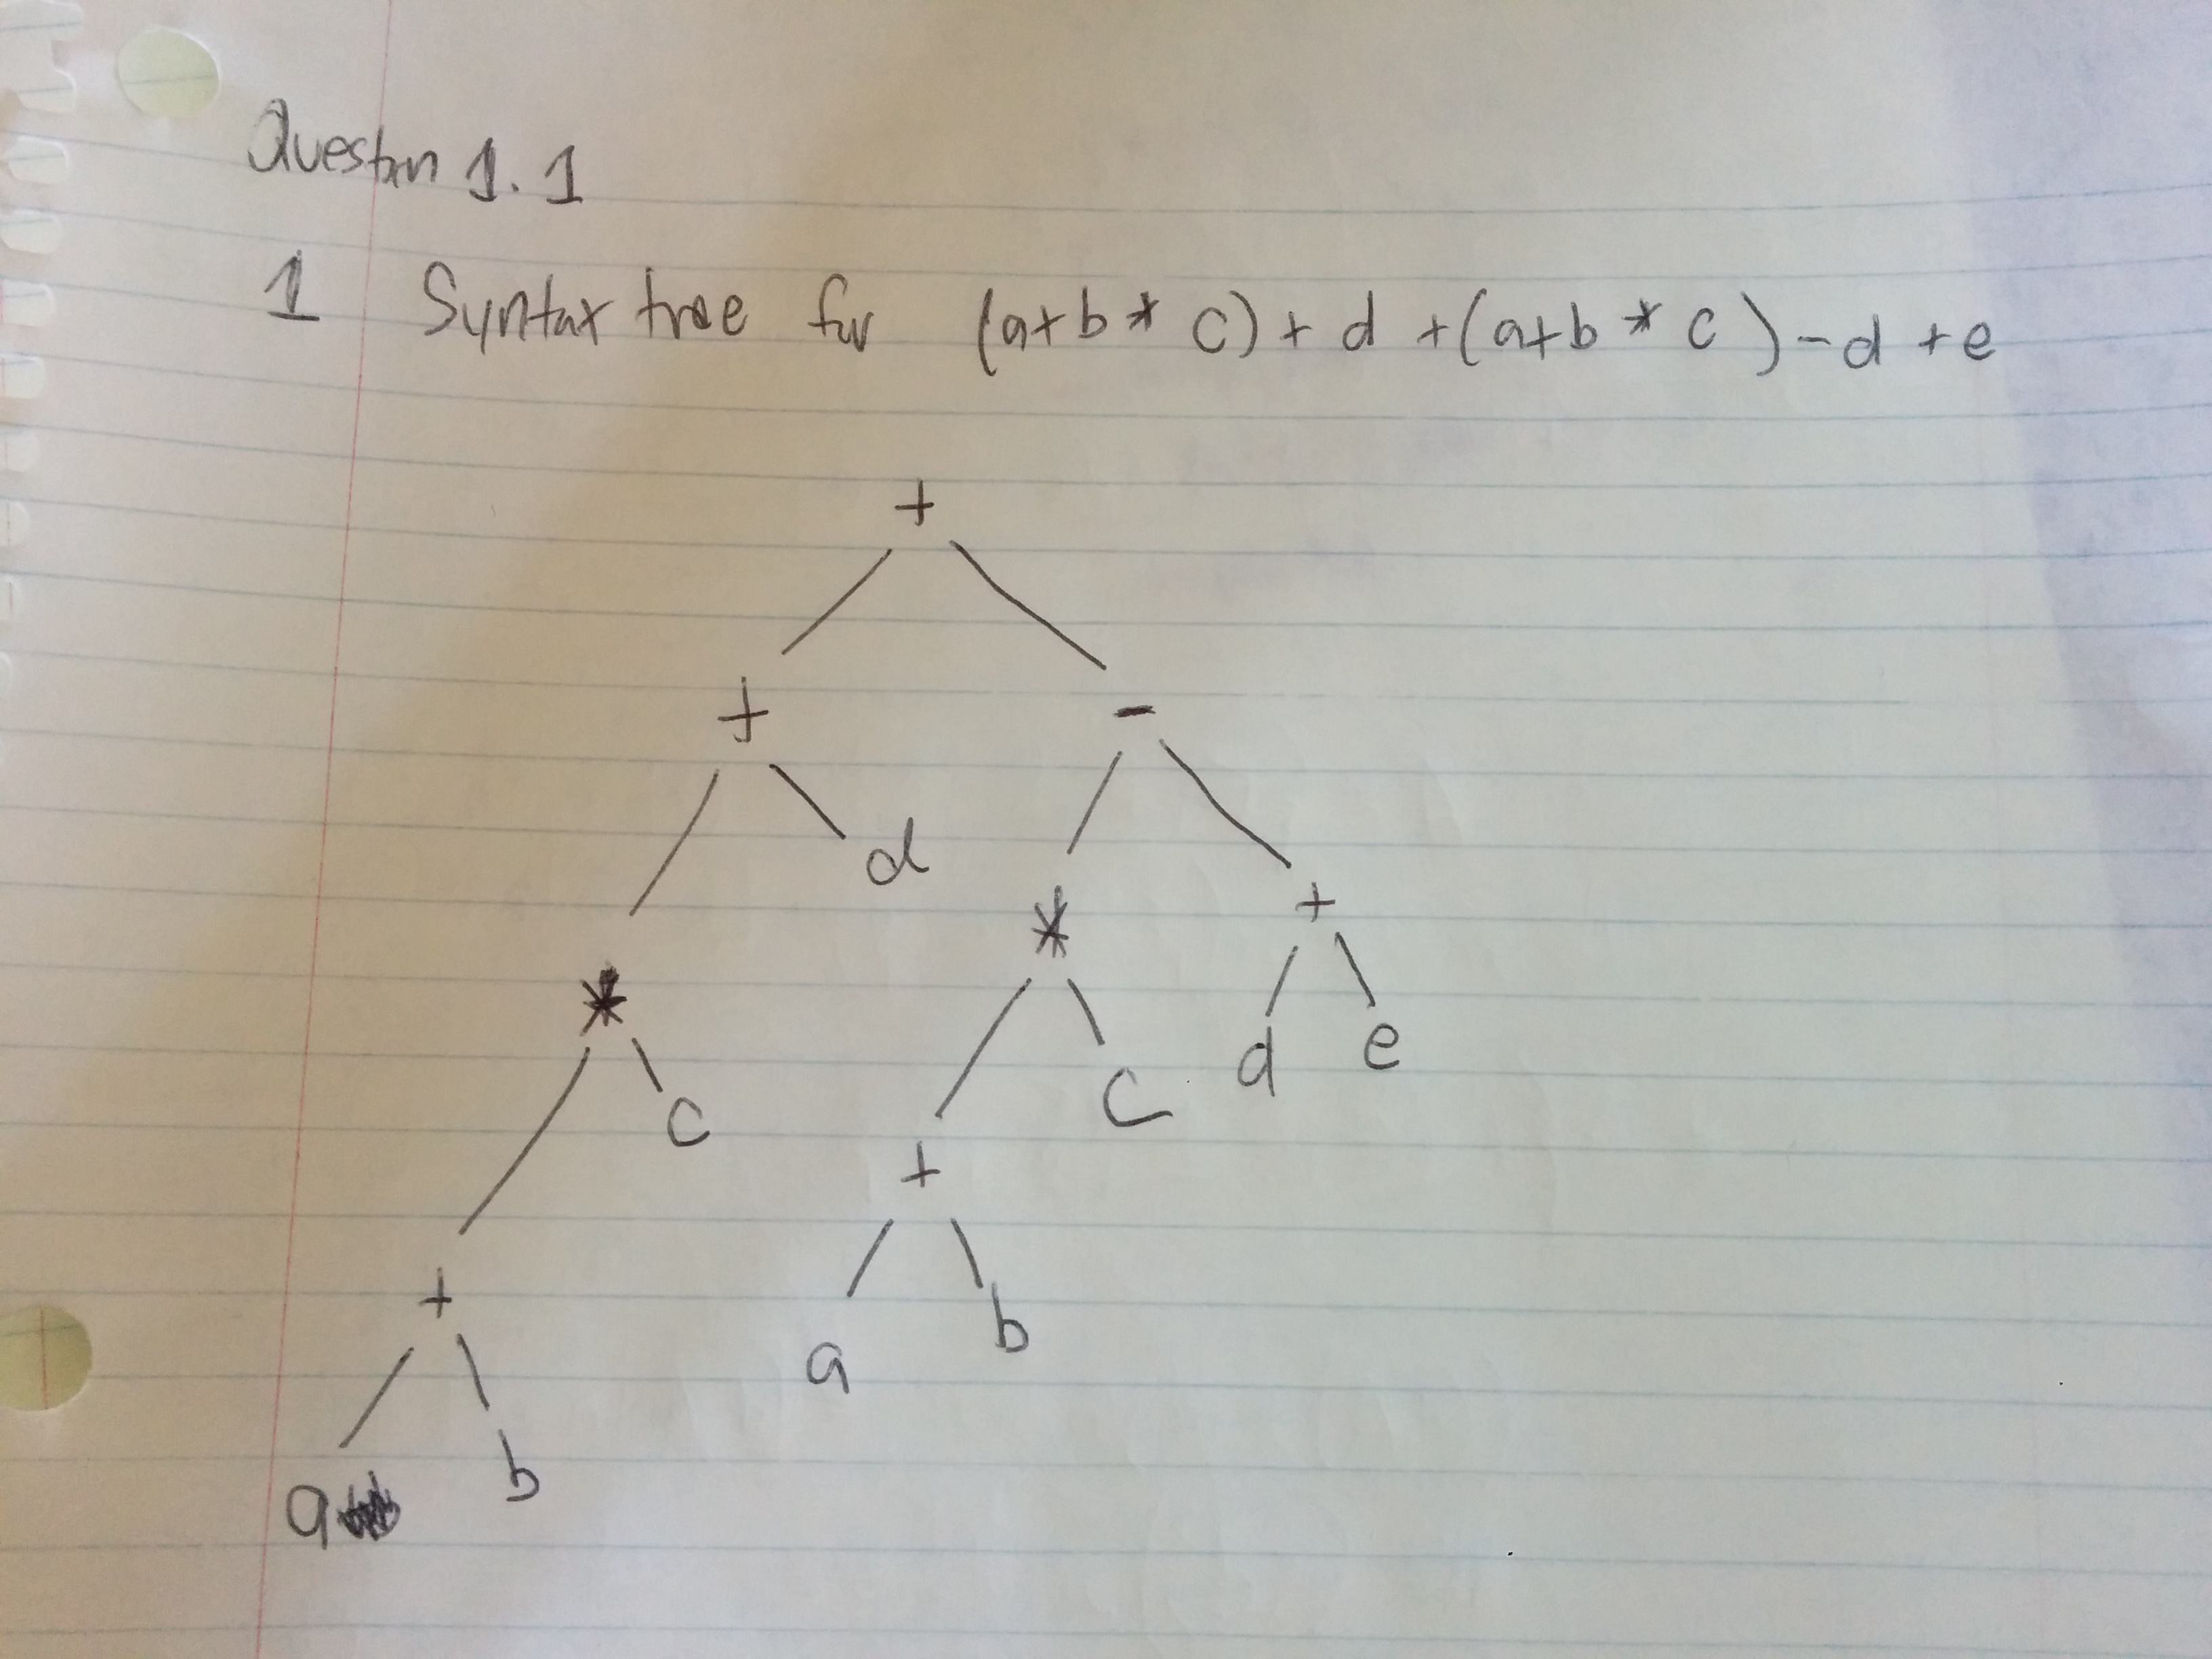
\includegraphics[scale=0.12]{IMG_20141025_154037.jpg}

\subsubsection{DAG (Directed Acyclic Graph) representation}
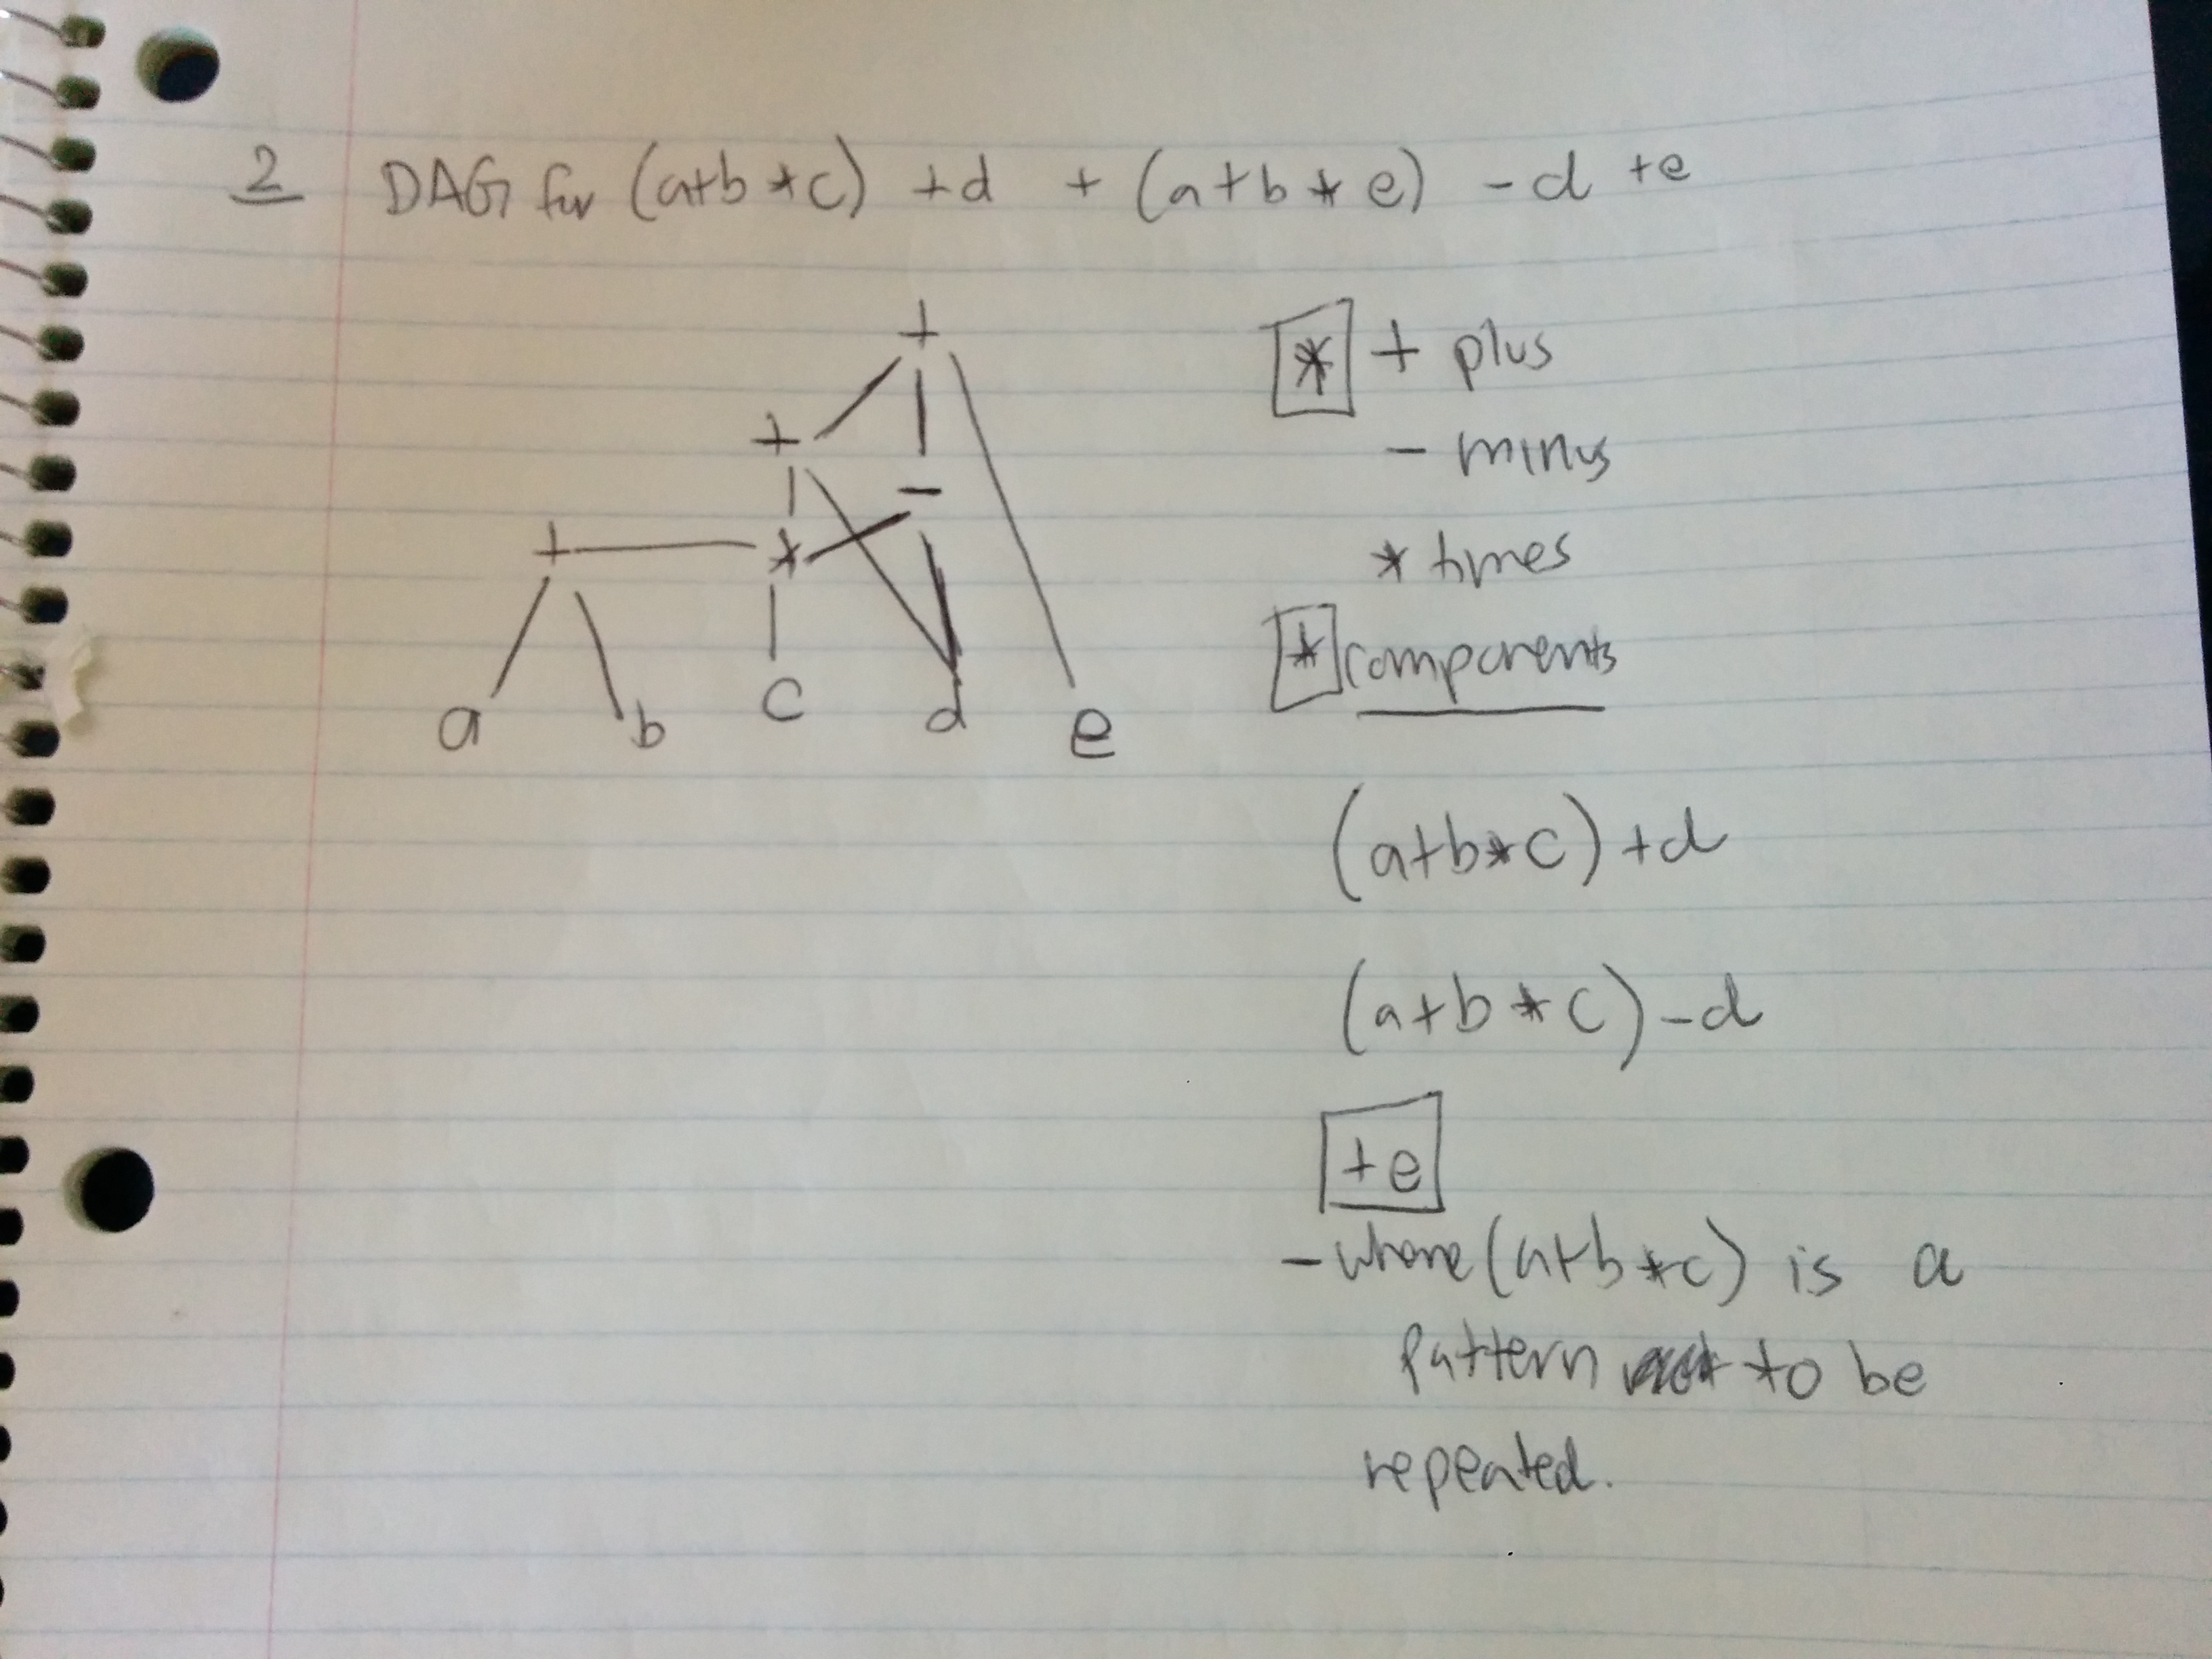
\includegraphics[scale=0.12]{IMG_20141025_154052.jpg}

\subsubsection{Three-Address Code representation}
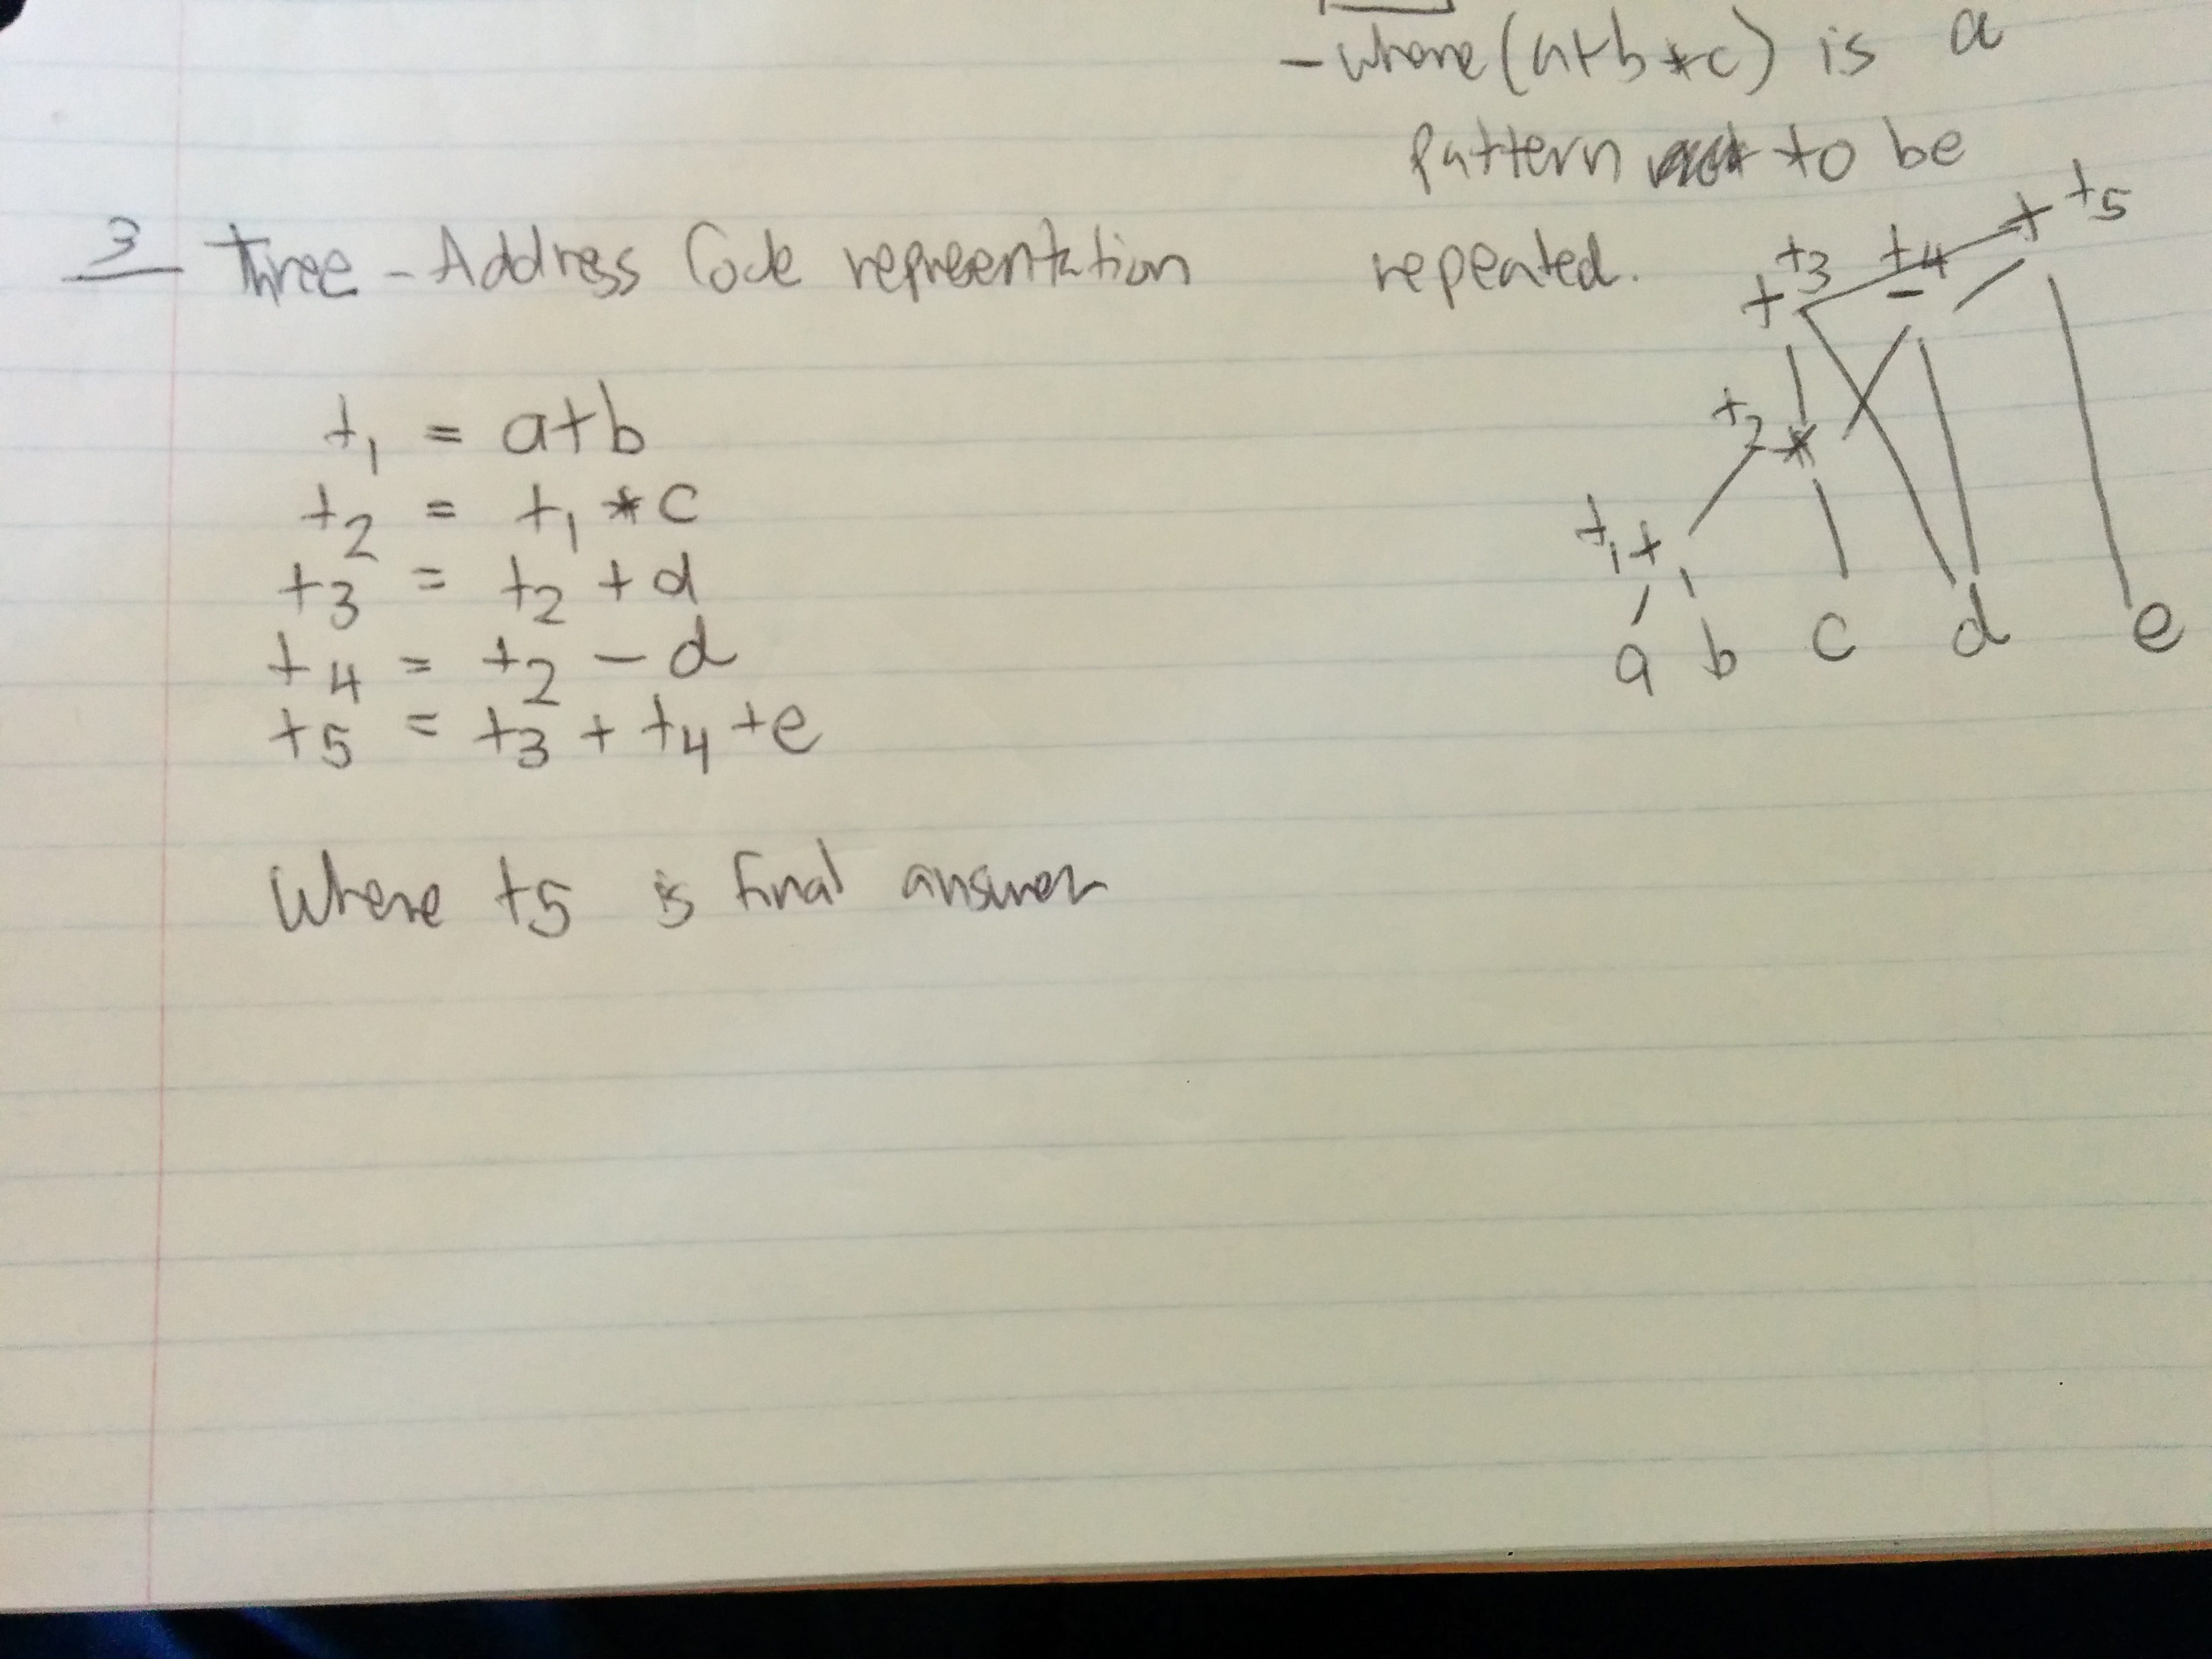
\includegraphics[scale=0.12]{IMG_20141025_154609.jpg}

\subsection{Question 1.2}

\subsubsection{Syntax Tree}
\par Please change the word "minus" to an actual minus (-) (My mistake I looked at this later) \\
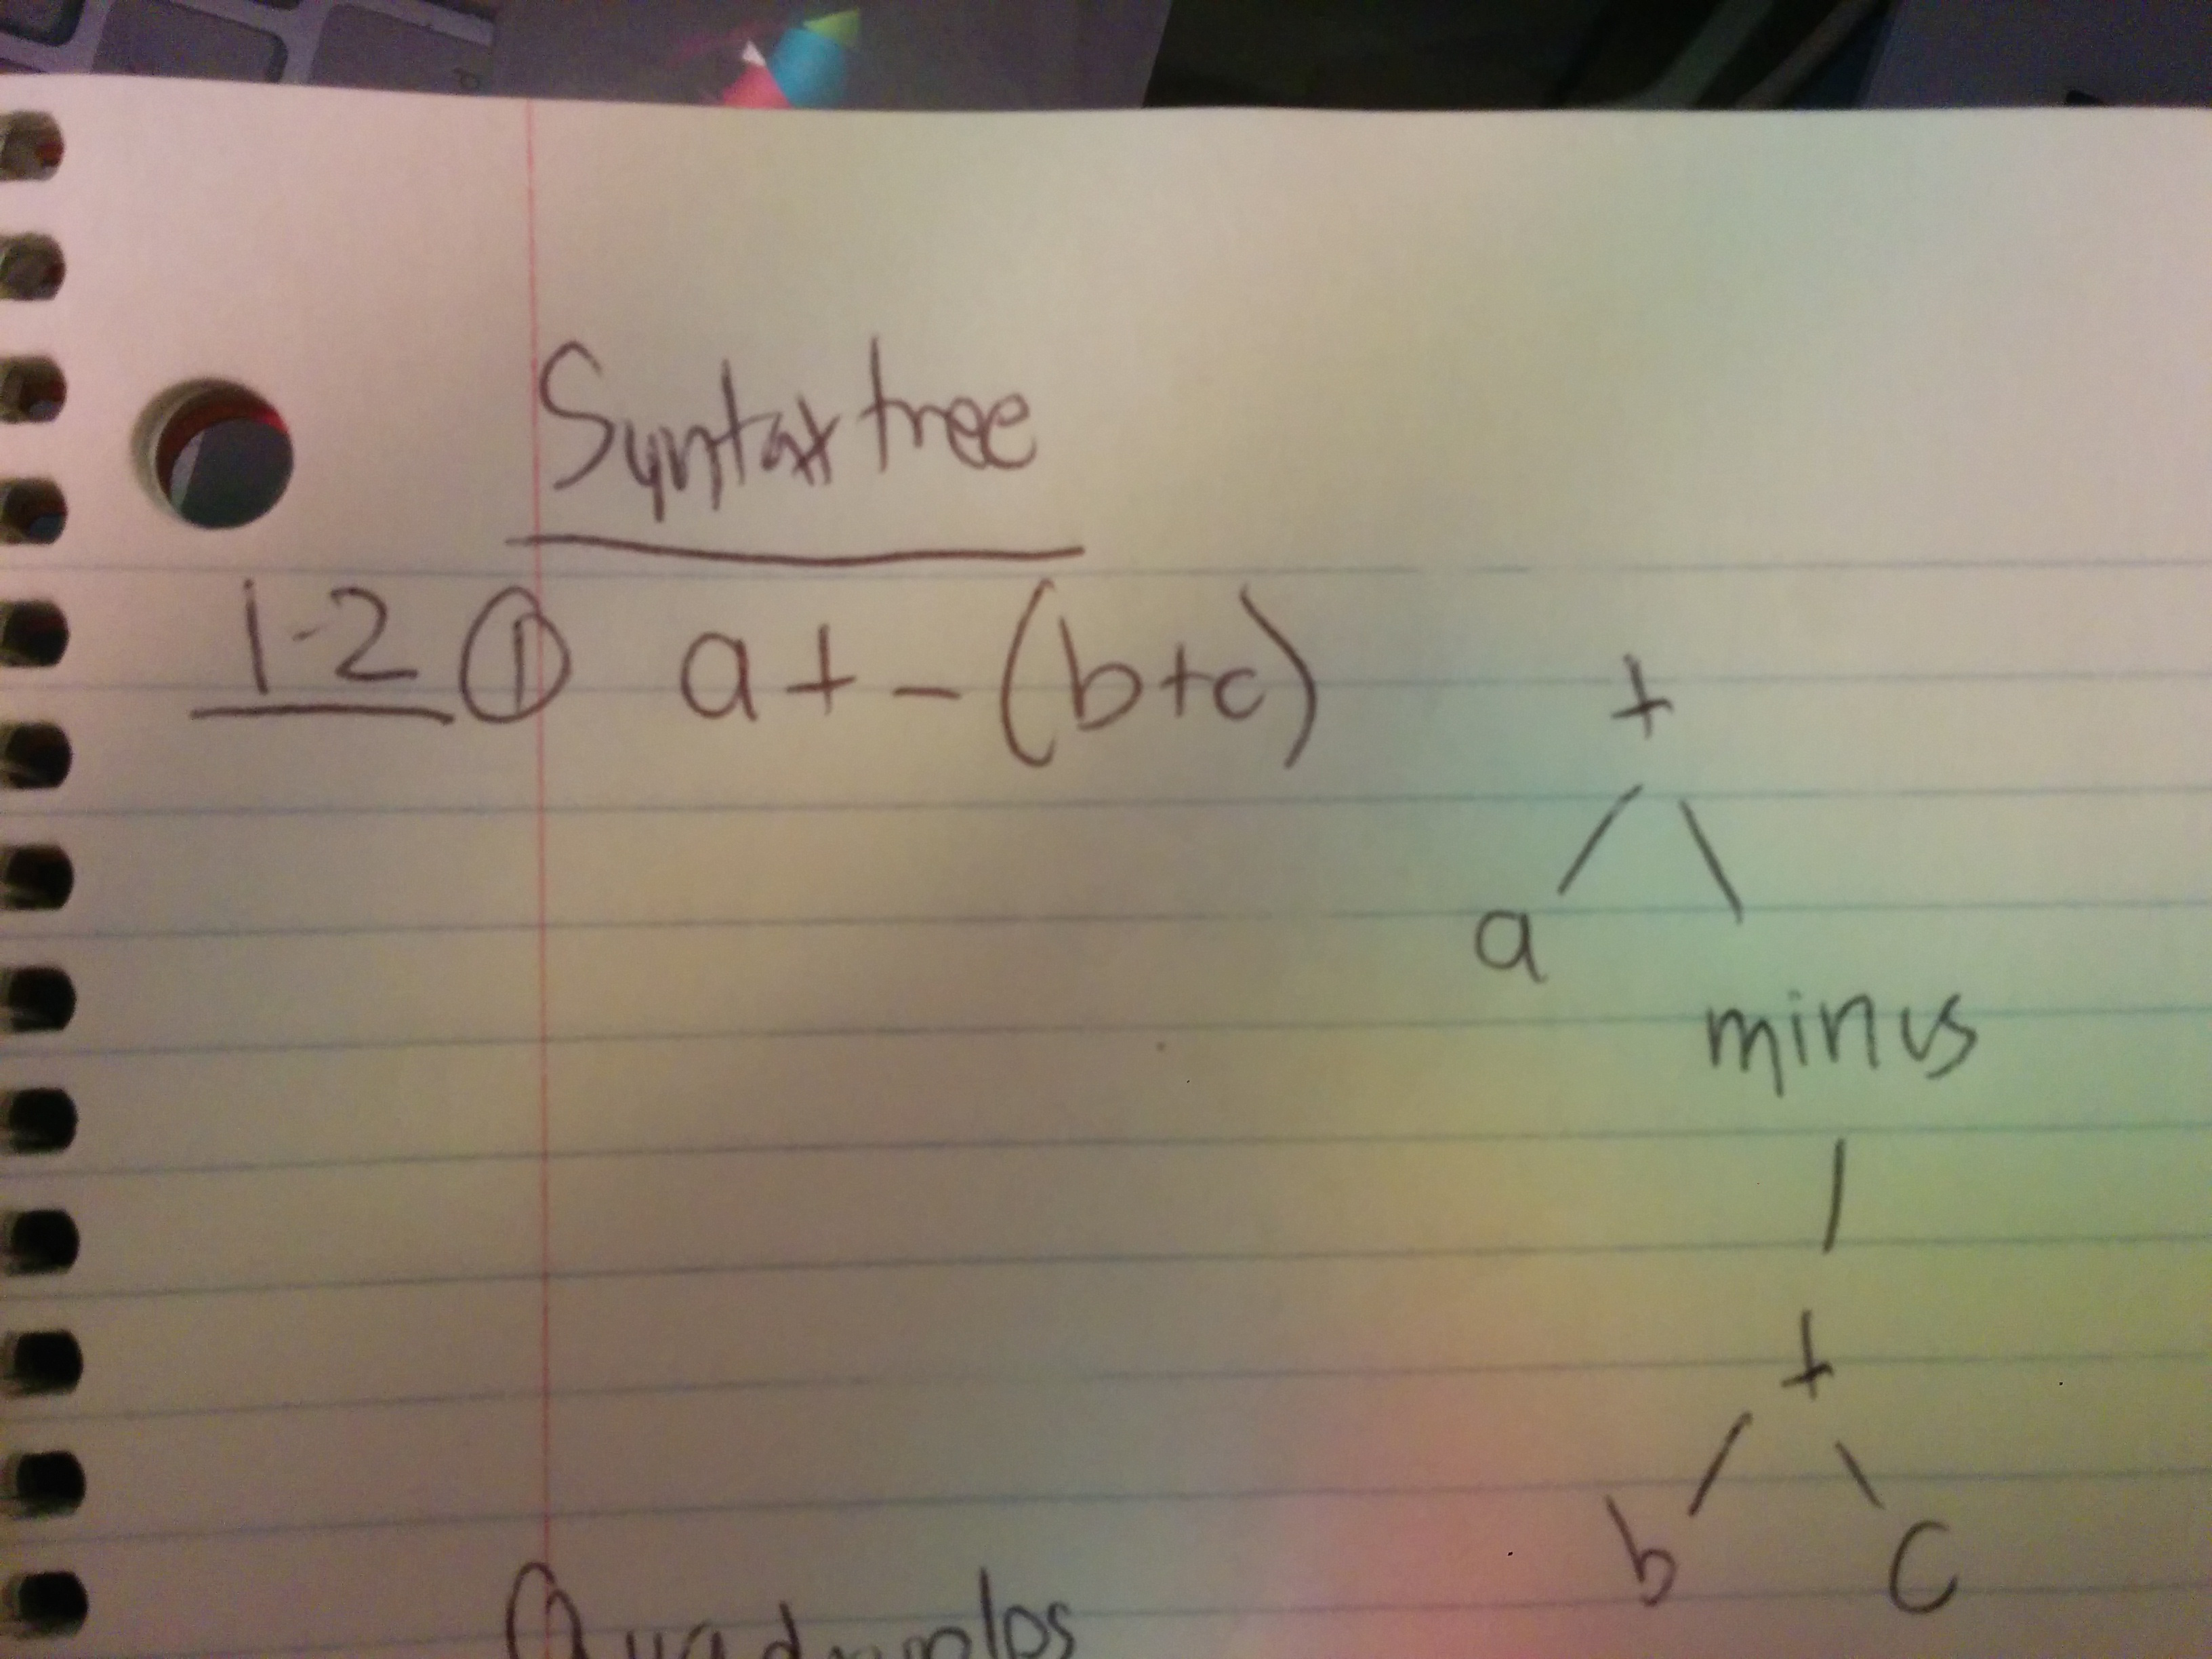
\includegraphics[scale=0.12]{IMG_20141028_235513.jpg}

\subsubsection{Quadruples}
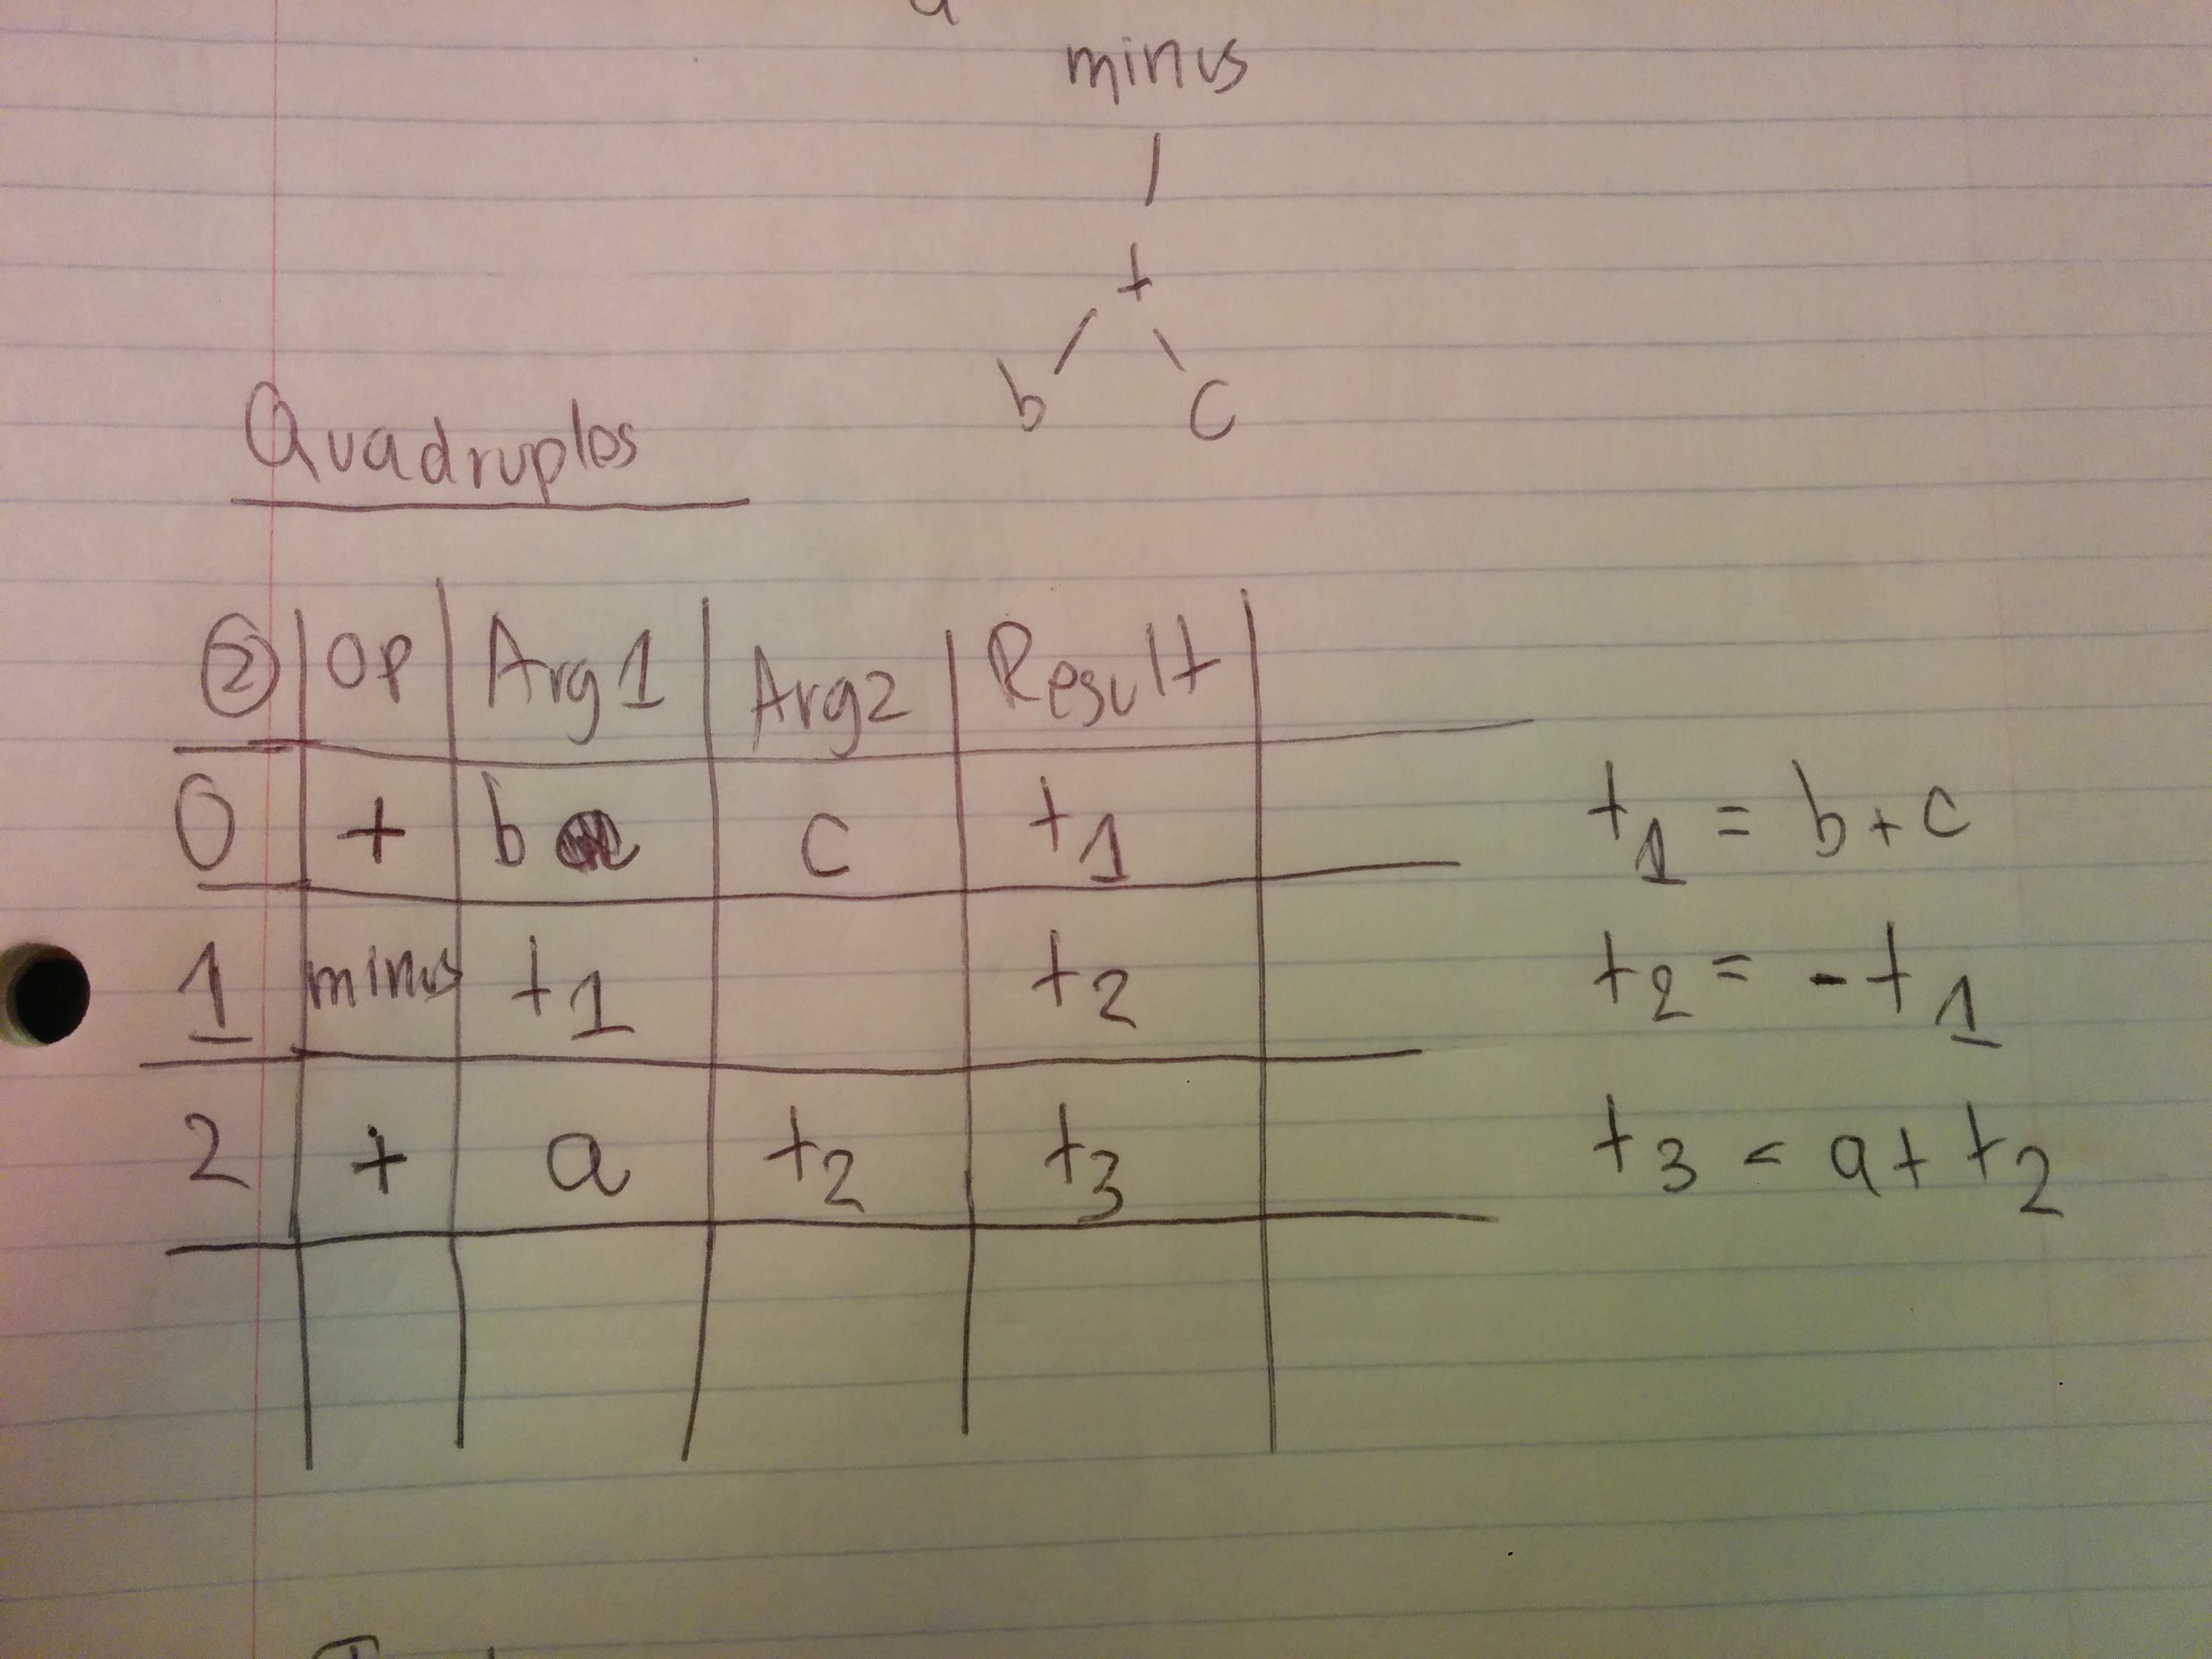
\includegraphics[scale=0.12]{IMG_20141028_235505.jpg}

\subsubsection{Triples}
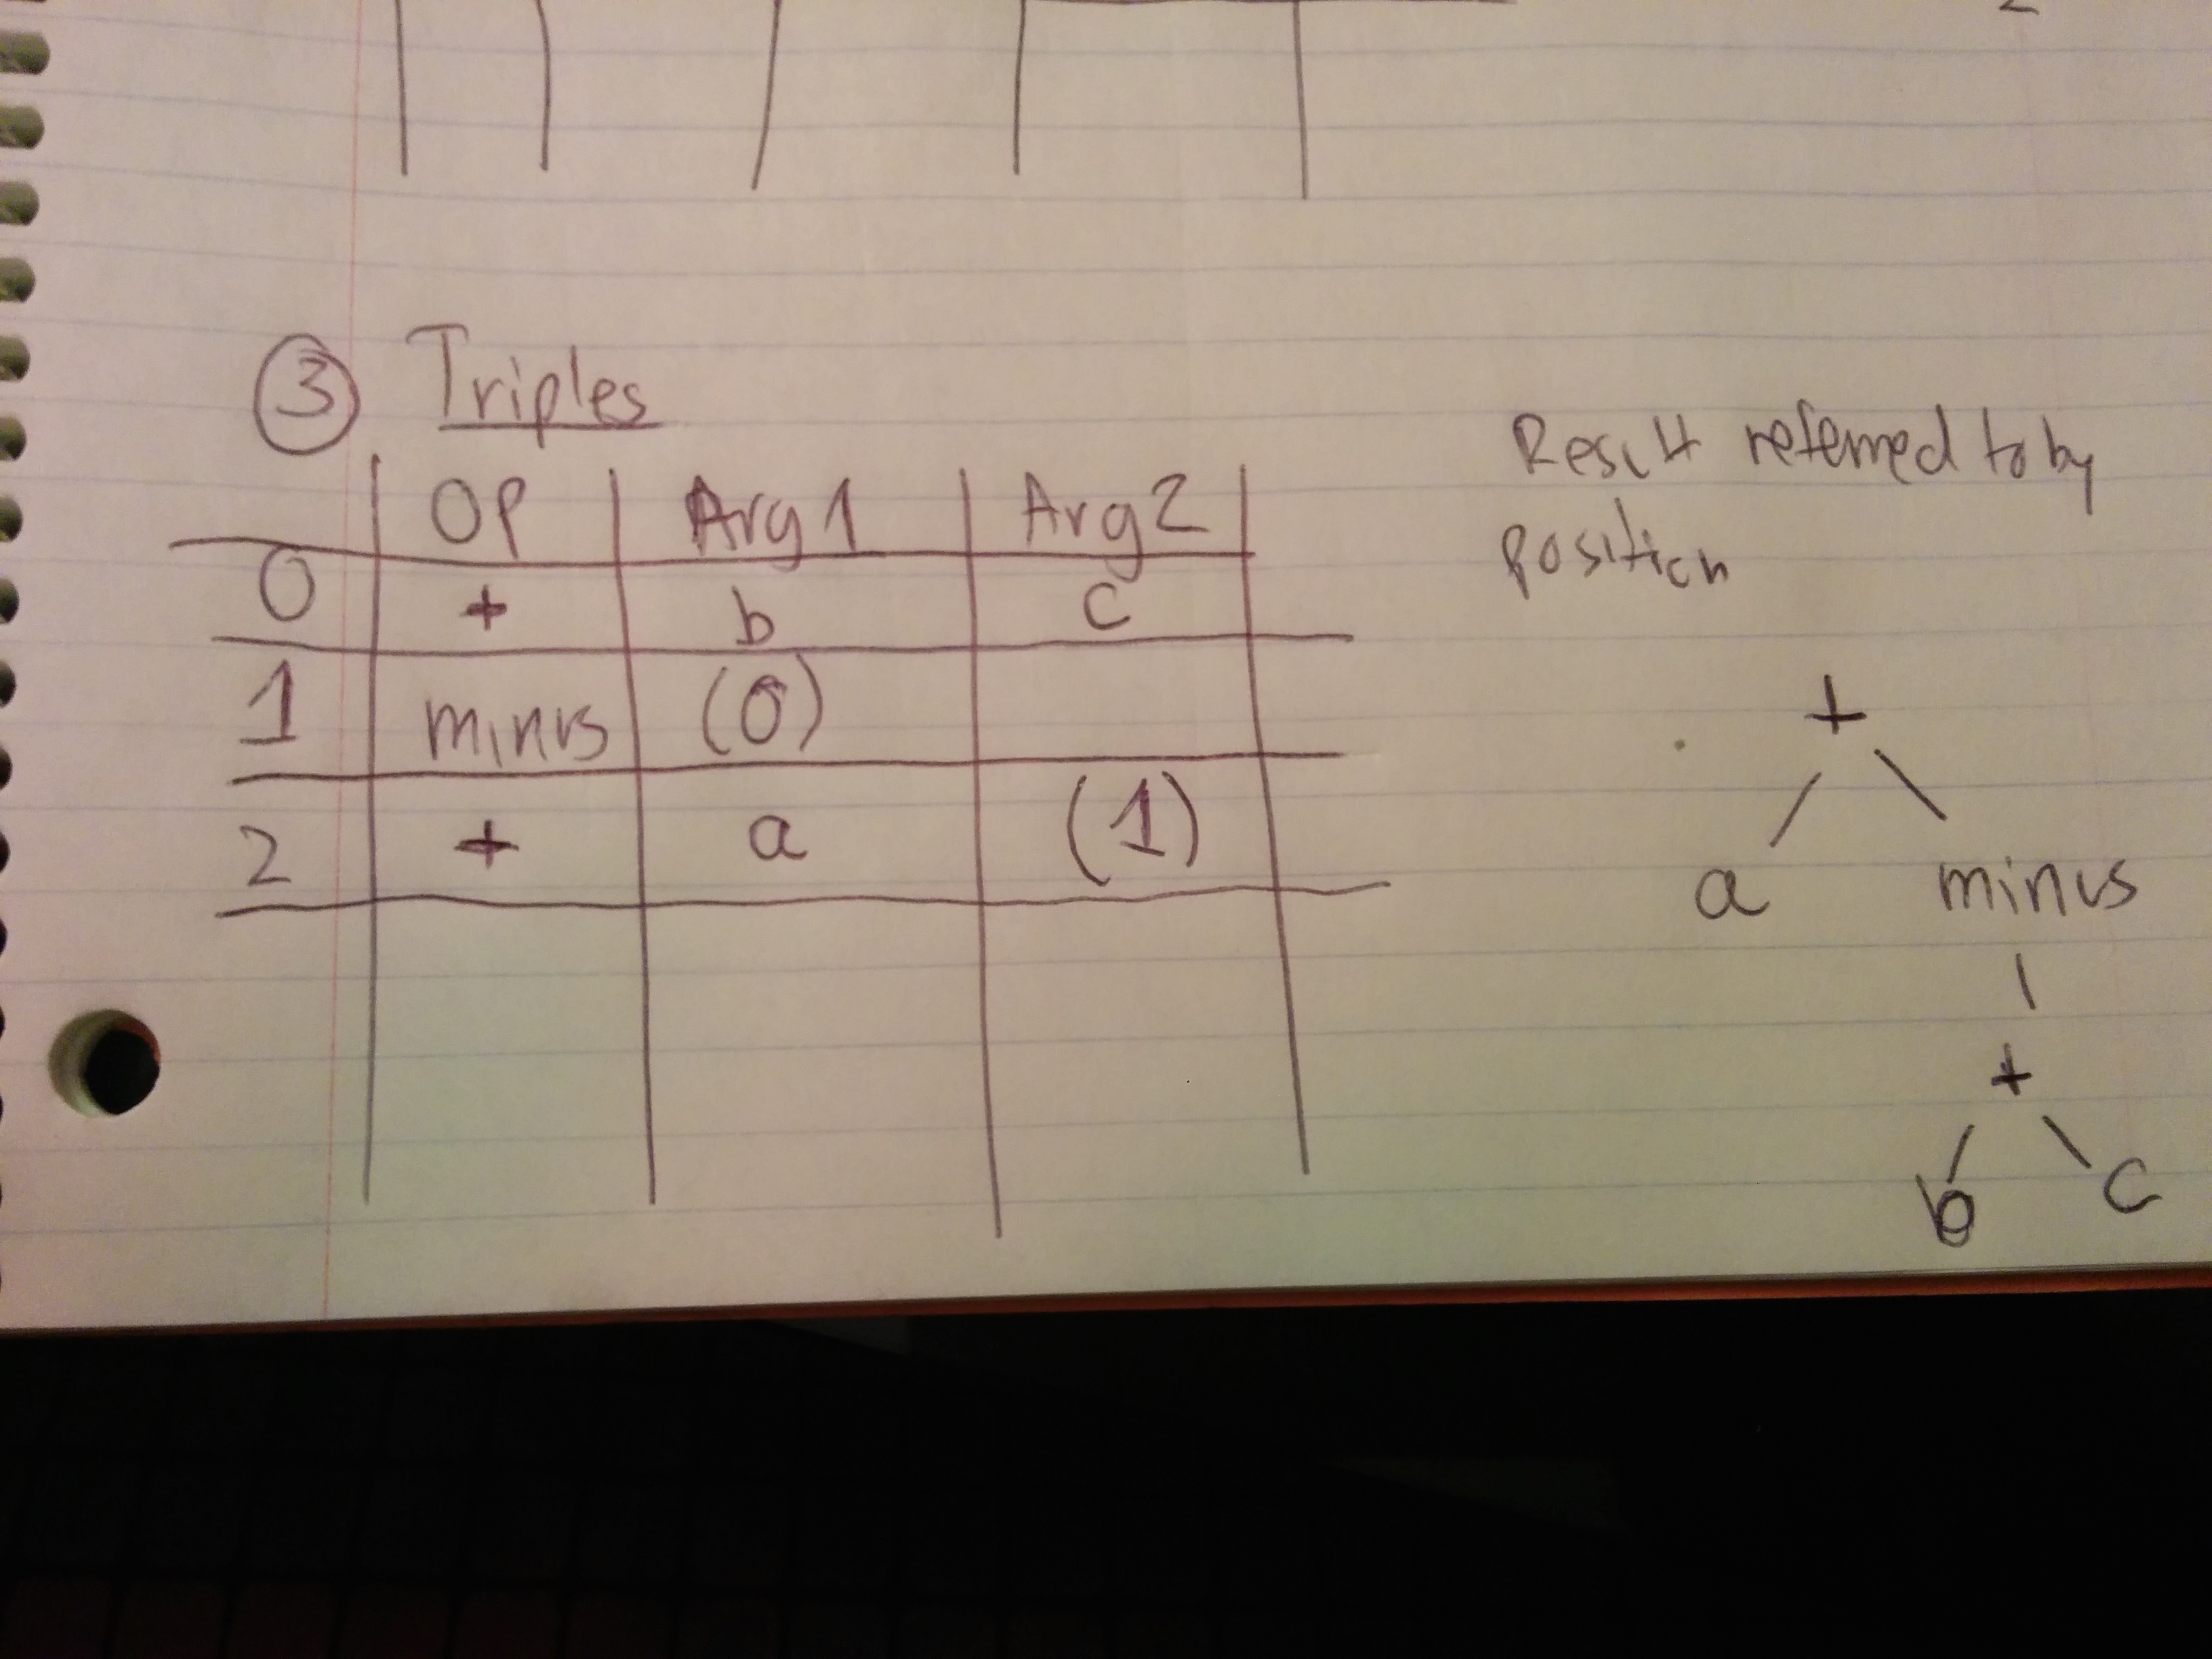
\includegraphics[scale=0.12]{IMG_20141028_235519.jpg}

\newpage

\subsubsection{Indirect Triples}
\par Please change the 35, 36, 37 to 0, 1, 2 instead as that's arbitrary and I misunderstood it on the slides. \\
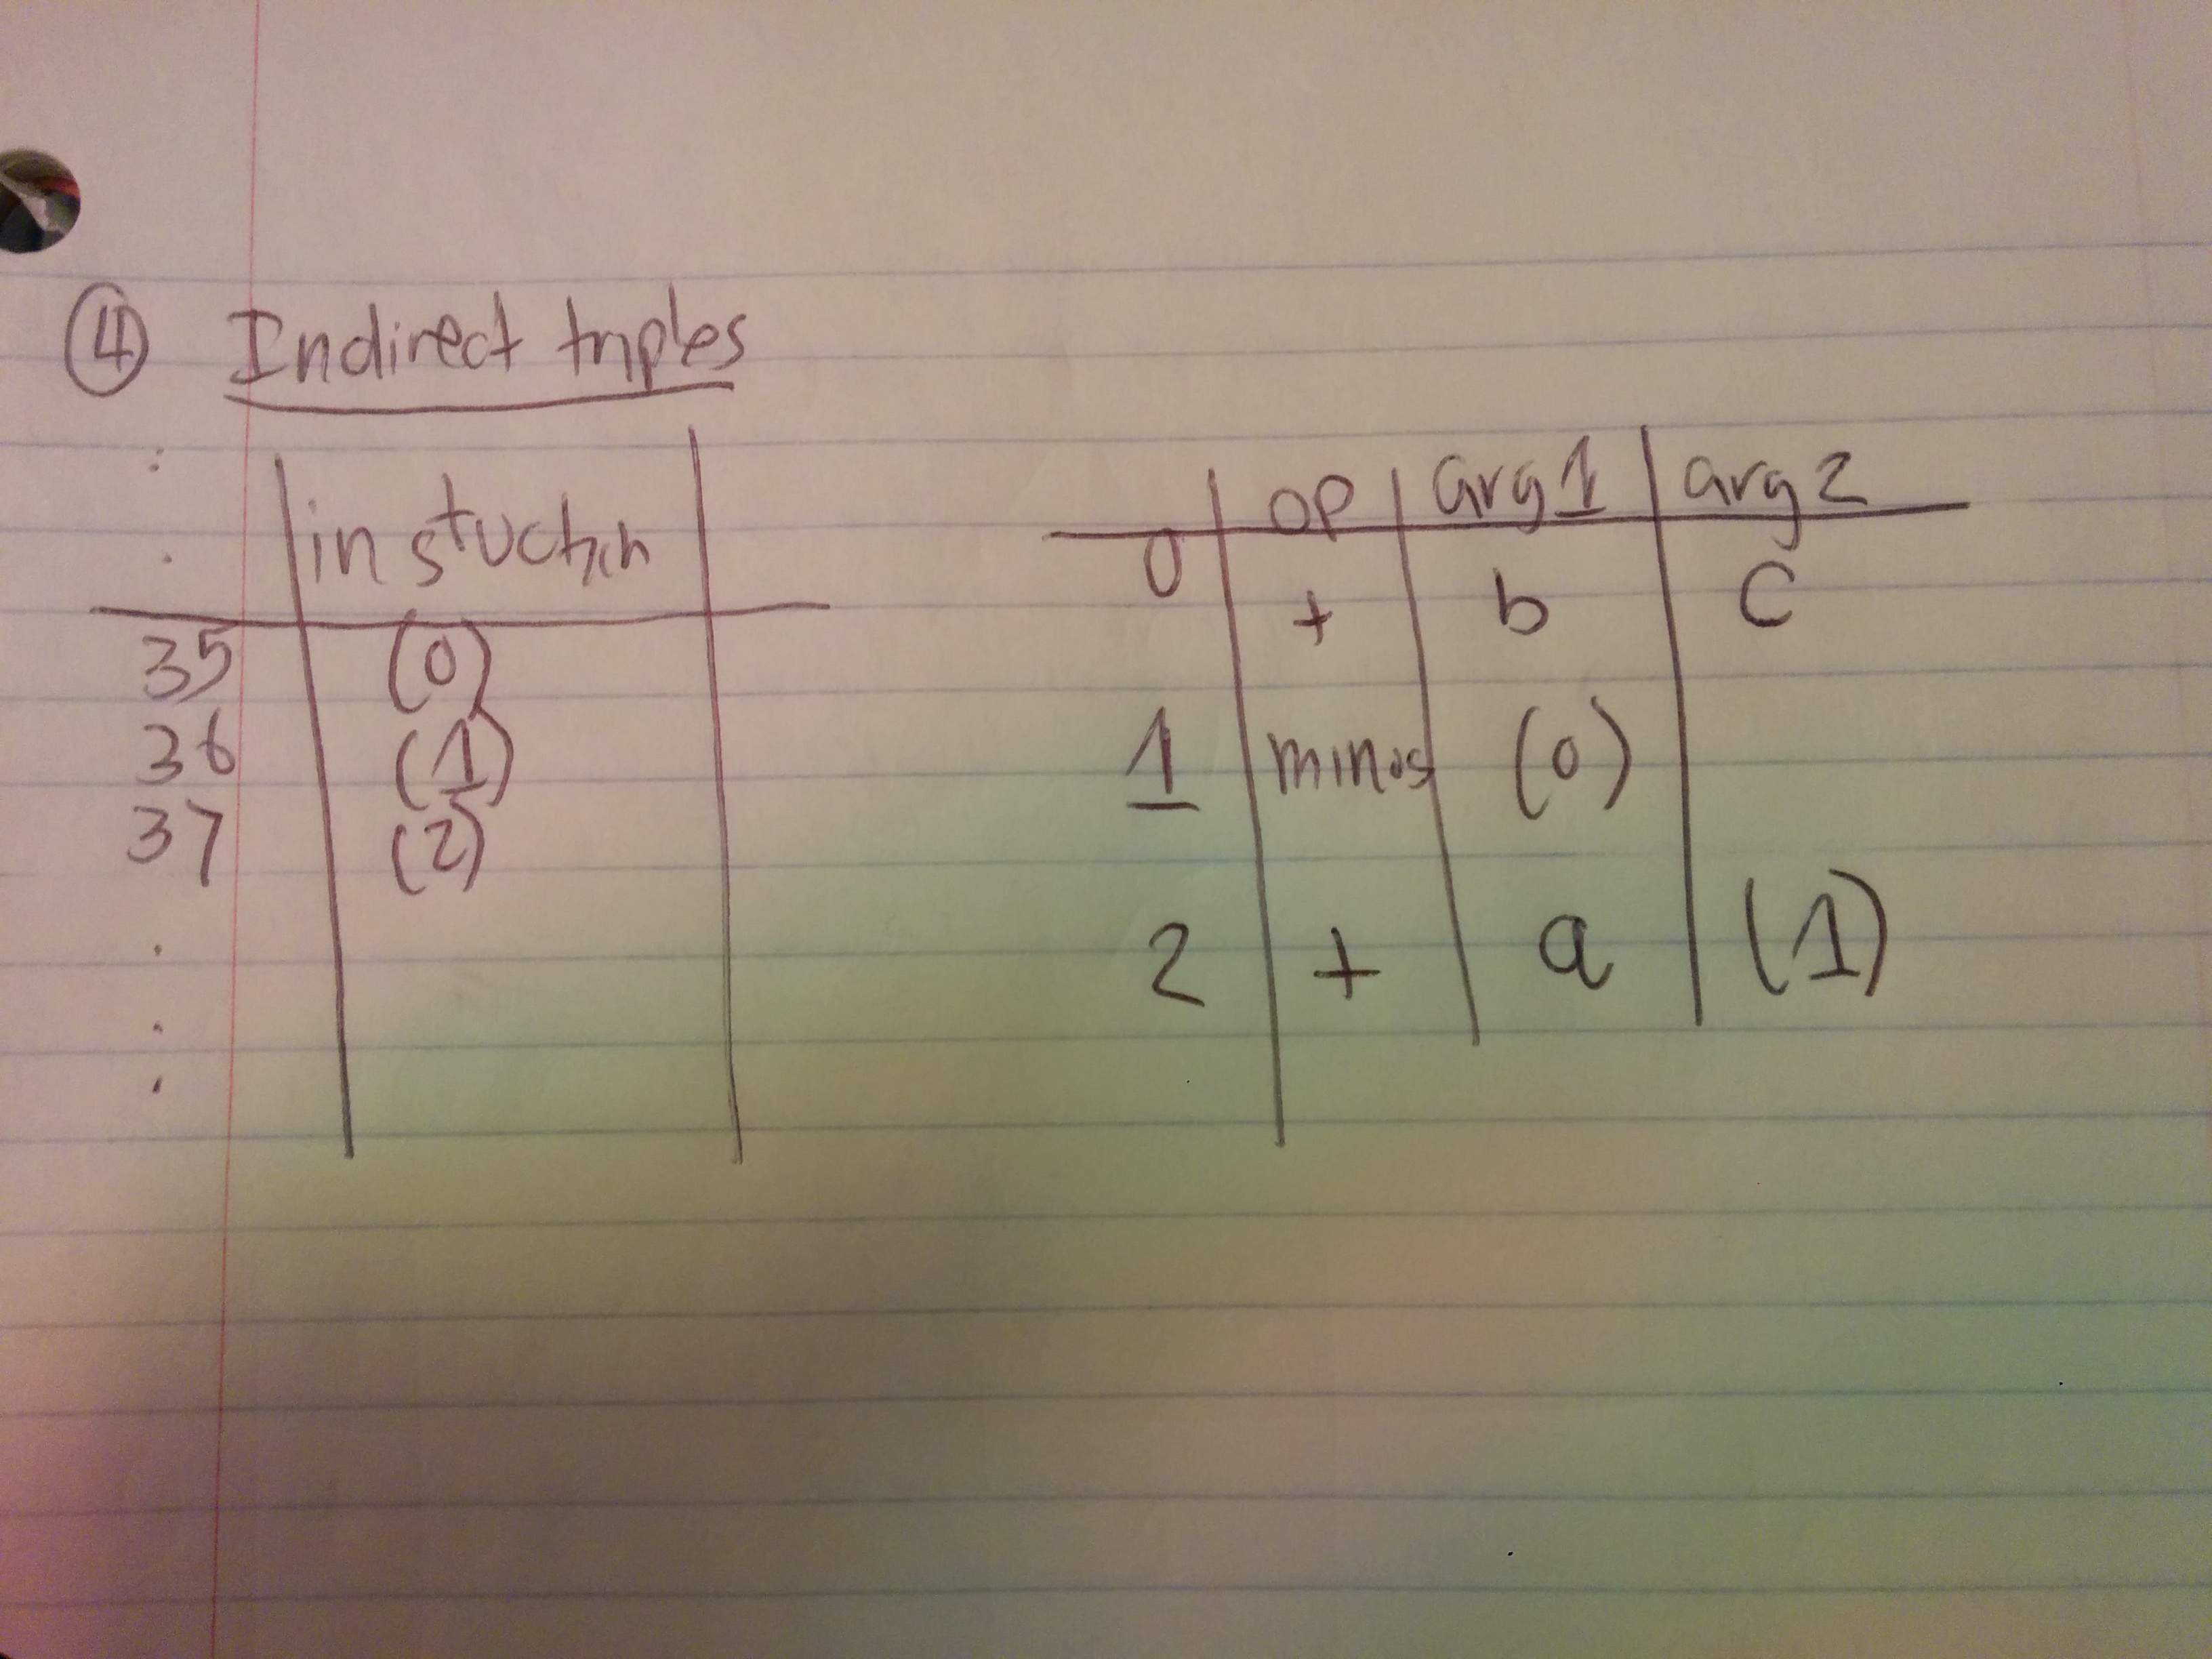
\includegraphics[scale=0.12]{IMG_20141029_001005.jpg}

\newpage

\section{Translation}

\subsection{Question 2.1}

\subsubsection{Add a translation rule for the following expression production: \\ E $\rightarrow$ E1 * E2}
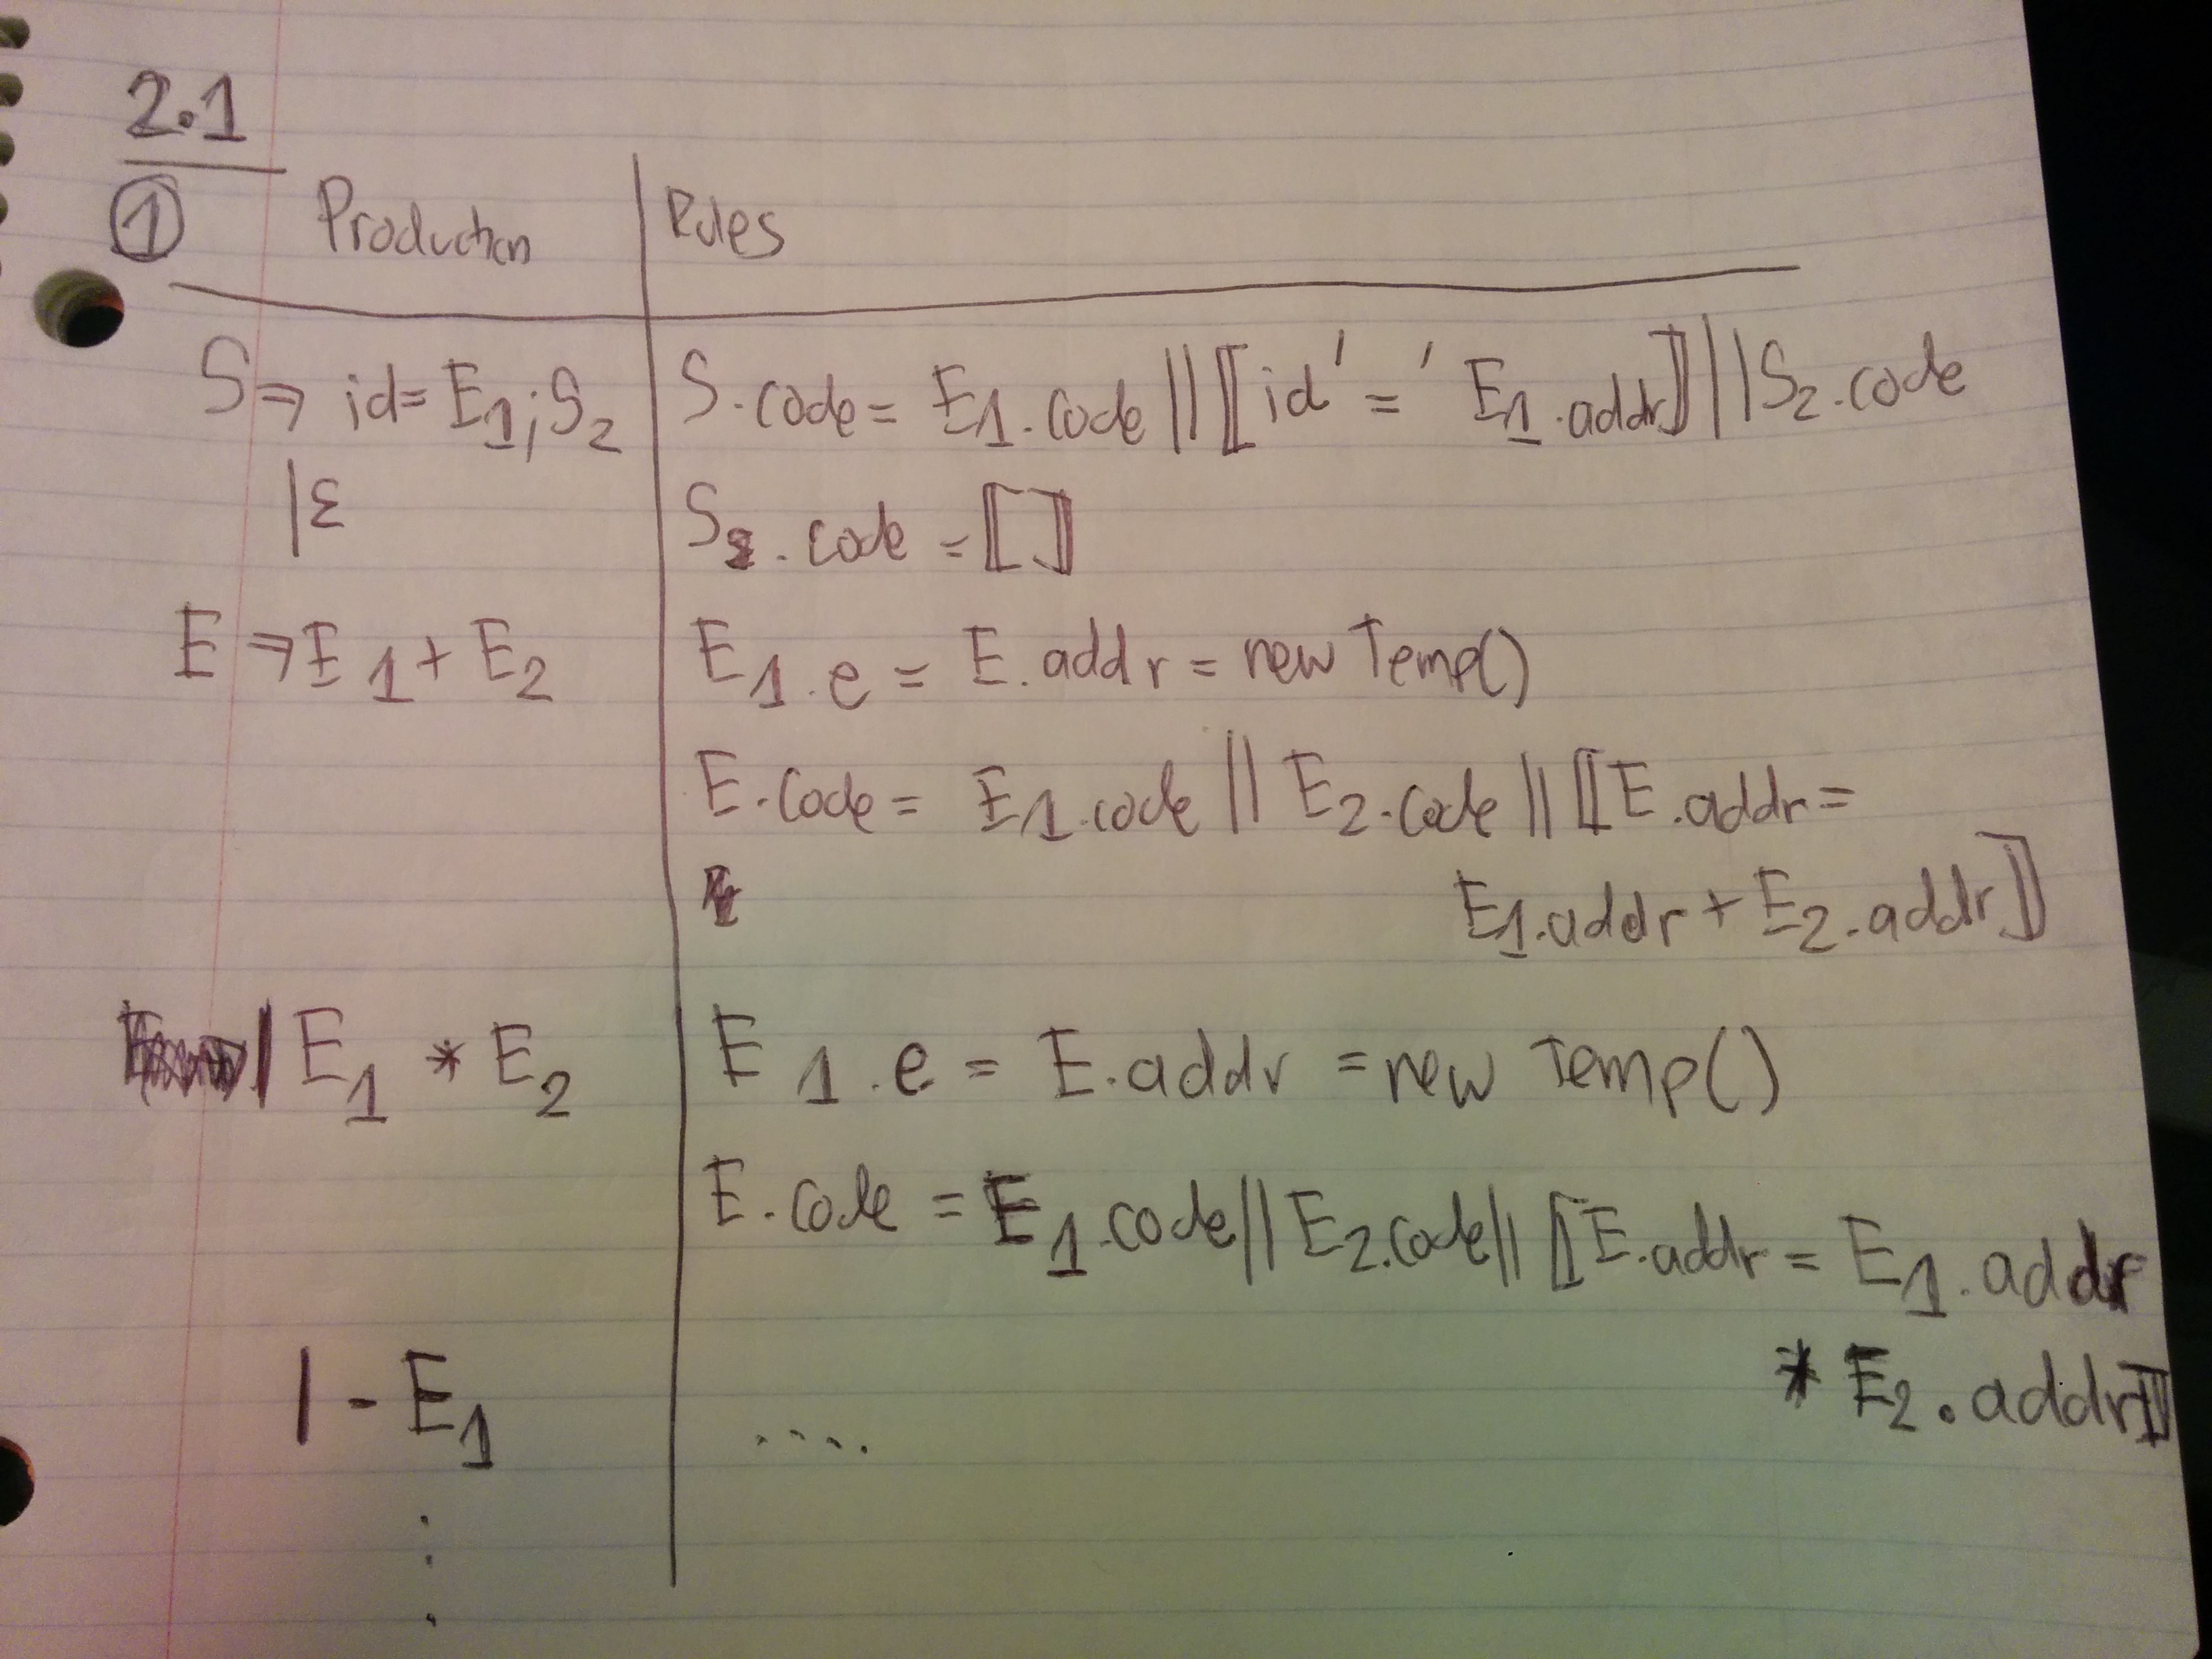
\includegraphics[scale=0.12]{IMG_20141029_003207.jpg}

\subsection{Question 2.2}
\subsubsection{Explain how the code is expected to evaluate, assuming parameters are passed call-by-value.}
\par Taken from the slides: If parameters are passed call-by-value then the contract is: 
\par $E_1$.code, ..., $E_n$.code are evaluated before results placed into temporary 
\par $E_1$.addr, ..., $E_n$.addr
\par \noindent The values are taken in as parameters, and the code is executed before you change or put the values into the add temporarily. For example, if the param you take in is 2, 2 and your code's execution is $param_1$ + $param_2$, then you would place the 4 into the $E_1$.addr after you've completed execution for $E_1$.code.

\subsection{Question 2.3}
\subsubsection{S $\rightarrow$ for(S1; B; S2) S3 \\ Extending the code from the book}
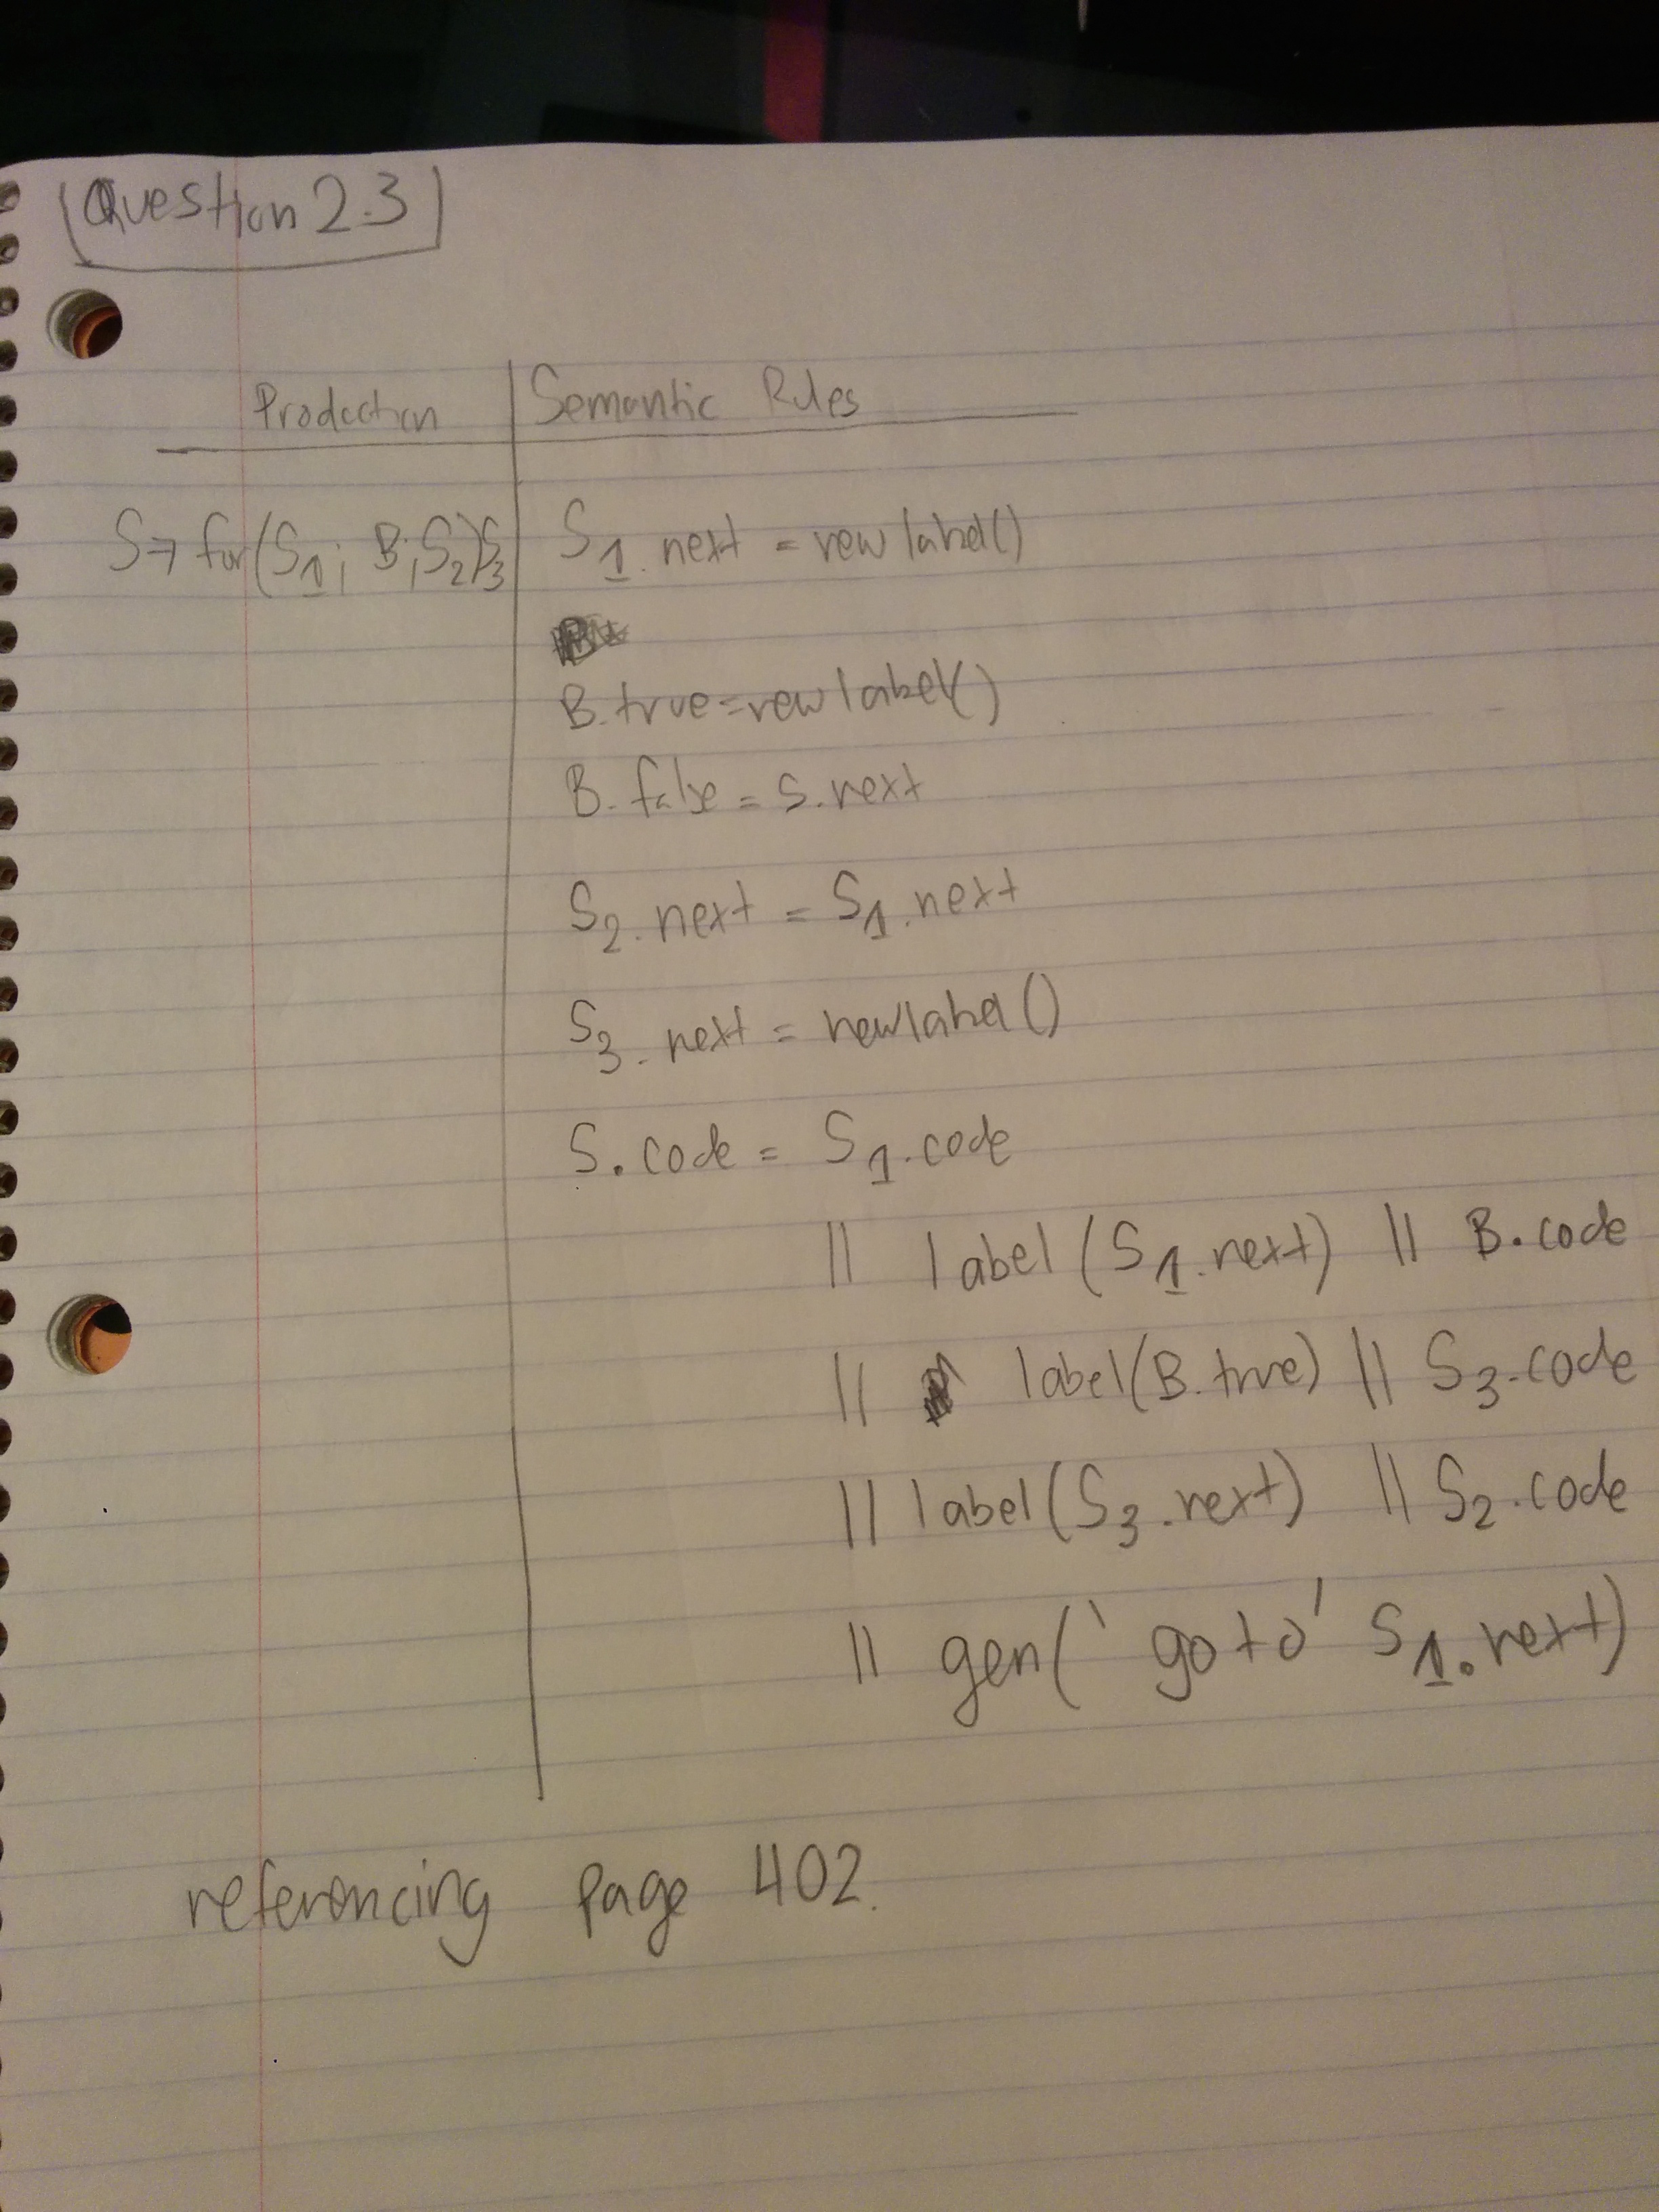
\includegraphics[scale=0.12]{IMG_20141029_014044.jpg}

\newpage

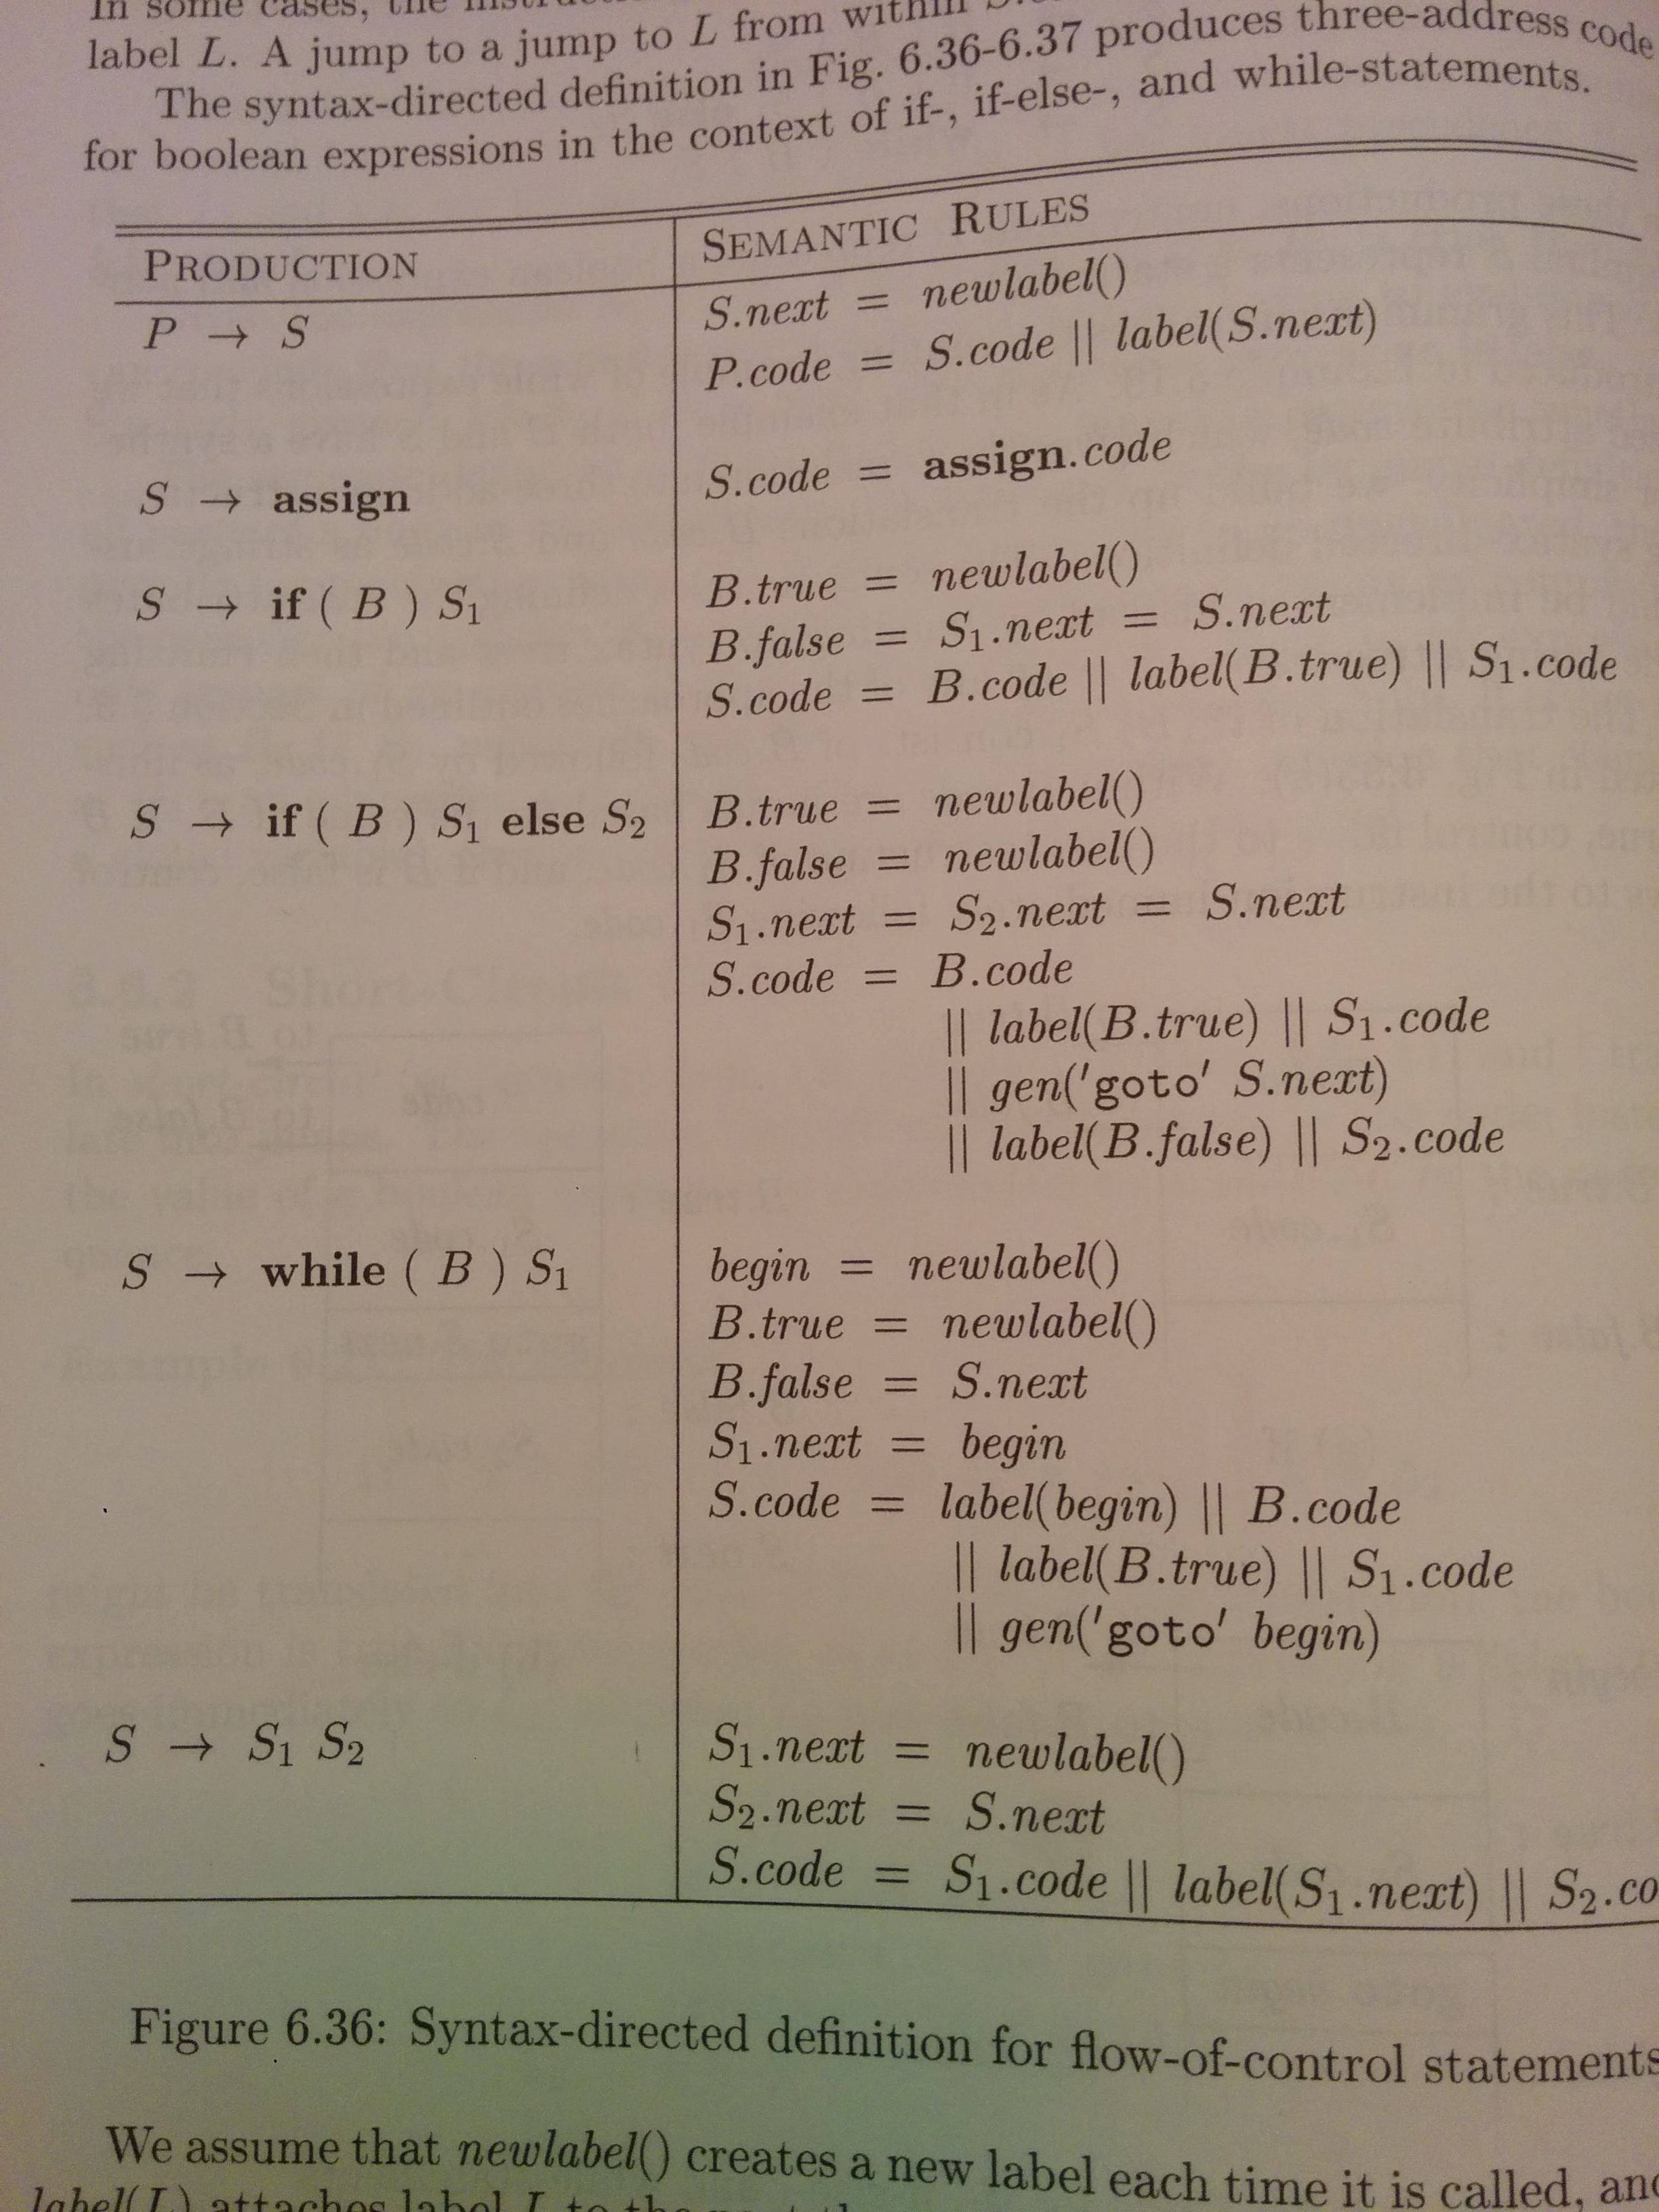
\includegraphics[scale=0.12]{IMG_20141029_013718.jpg}

\end{document}  